%!TEX root=../GaugeCNNTheory.tex


\newpage


\begin{figure}
	\centering
	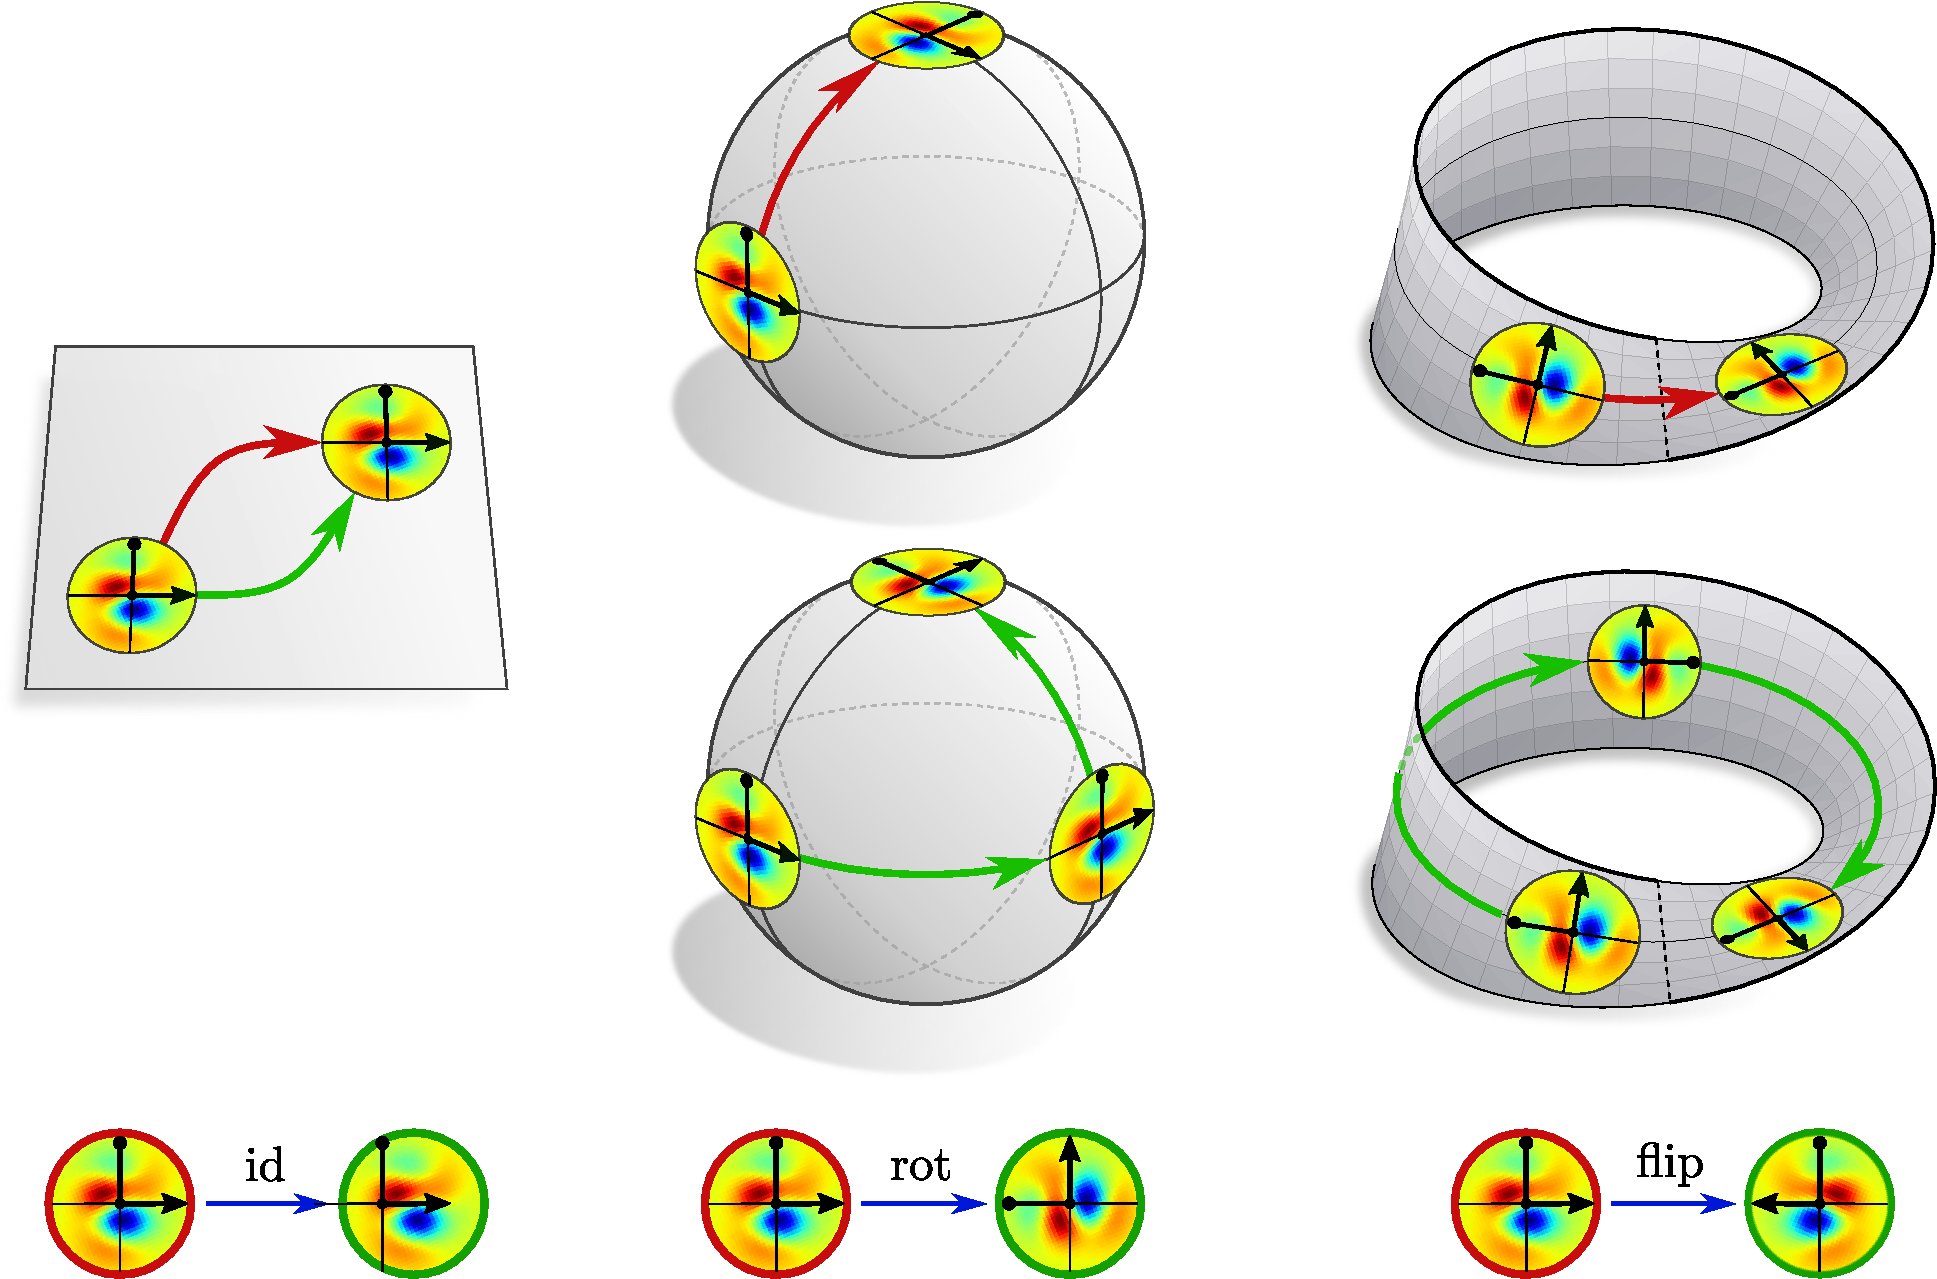
\includegraphics[width=.93\columnwidth]{figures/intro_transport_ambiguity.pdf}
	\caption{\small
		درک شهودی از ابهام ذاتی اشتراک وزن روی منیفولدها.
		\ \ \emph{چپ:}
		تفسیر رایج اشتراک وزن روی صفحه، جابجایی یک کرنل روی کل فضا است.
		از آنجا که انتقال موازی روی فضاهای مسطح مستقل از مسیر است، این امر مبهم نیست.
		\ \ \emph{وسط:}
		روی فضاهای خمیده، مانند کره، انتقال موازی وابسته به مسیر است.
		مسیرهای مختلف منجر به کرنل‌هایی می‌شوند که نسبت به یکدیگر چرخیده هستند.
		\ \ \emph{راست:}
		نوار موبیوس منیفولدی غیرقابل جهت‌یابی است.
		بنابراین مسیرهای مختلف می‌توانند منجر به کرنل‌هایی شوند که نسبت به یکدیگر منعکس هستند.
		\ \ \emph{پایین:}
		ما تراز مختلف کرنل‌ها را با انتخاب‌های مختلف چارچوب‌های مرجع محلی فضاهای مماس متناظر رسمی می‌کنیم.
		معلوم است که هیچ انتخابی از چارچوب‌های مرجع (گیج) روی منیفولدهای عمومی ترجیح داده نمی‌شود.
		مختصاتی‌سازی‌های مختلف توسط تبدیل‌های گیج مرتبط هستند که مقادیری در گروه ساختار \lr{$G$} منیفولد می‌گیرند (گروه بدیهی \lr{$G=\{e\}$} برای صفحه، گروه چرخش \lr{$G=\SO2$} برای کره و گروه انعکاس \lr{$G = \Flip$} برای نوار موبیوس).
		\lr{CNN}های مستقل از مختصات ابهام چارچوب‌های مرجع را با اعمال کرنل‌های کانولوشن قابل هدایت \lr{$G$} (هم‌متغیر گیج) مورد توجه قرار می‌دهند.
	}
	\label{fig:weight_sharing_ambiguity}
\end{figure}


\section{مرور کلی و شهود بصری}
\label{sec:visual_intro}


فرمول‌بندی جبری \lr{CNN}های مستقل از مختصات نیاز به آشنایی با نظریه گروه، نظریه نمایش و هندسه دیفرانسیل دارد که ممکن است مانعی برای مخاطب غیرفنی باشد.
با این حال، اکثر ساختارها و نتایج ما از لحاظ هندسی بسیار شهودی هستند و می‌توانند با چند نمونه بصری توضیح داده شوند.
این بخش سعی می‌کند مروری کلی و شهود بصری در مورد \lr{CNN}های مستقل از مختصات ارائه دهد.

بخش زیر~\ref{sec:intro_overview_GM_conv} کانولوشن‌های مستقل از مختصات \lr{$\GM$} روی منیفولدهای ریمانی را معرفی می‌کند.
هم‌متغیری آنها تحت عمل ایزومتری‌ها در بخش~\ref{sec:intro_overview_isometry} بحث می‌شود.
بخش~\ref{sec:intro_overview_G_structure_choice} در مورد عواملی که بر انتخاب ساختار \lr{$G$} در طراحی \lr{CNN}های مستقل از مختصات تأثیر می‌گذارند، نظر می‌دهد.




\toclesslab\subsection{ساختارهای \lr{\textit{G}} و کانولوشن‌های مستقل از مختصات \lr{\textit{GM}}}{sec:intro_overview_GM_conv}
از آنجا که کانولوشن‌ها اساساً با خاصیت اشتراک وزن خود مشخص می‌شوند، سؤال اصلی در این کار این است:
\vspace*{-1ex}
\begin{center}\it
	کرنل‌های کانولوشن چگونه باید روی منیفولدهای ریمانی به اشتراک گذاشته شوند؟
	\footnote{
		این سؤال به طور کلی‌تر به هر تابع قالب محلی، برای مثال بایاس‌ها یا غیرخطی‌های نقطه‌ای، اعمال می‌شود.
	}
\end{center}

%%%%%%%%%%%%%%%%%%%%%%%%%%%%%%%%%%%%%%%%%%%%%%%%%%%%%%%%%%%%%%%%%%%%%%%
%%%%%%%%%%%%%%%%%%%%%%%%%%%%%%%%%%%%%%%%%%%%%%%%%%%%%%%%%%%%%%%%%%%%%%%
\marginnote{} % somehow forces stuff on first page...
%%%%%%%%%%%%%%%%%%%%%%%%%%%%%%%%%%%%%%%%%%%%%%%%%%%%%%%%%%%%%%%%%%%%%%%
%%%%%%%%%%%%%%%%%%%%%%%%%%%%%%%%%%%%%%%%%%%%%%%%%%%%%%%%%%%%%%%%%%%%%%%


یک رویکرد رایج \marginnote{اشتراک وزن از طریق تقارن‌ها} اشتراک وزن‌ها از طریق عمل گروه تقارن فضای زیربنایی است~\cite{Cohen2016-GCNN,Kondor2018-GENERAL}.
برای مثال، \lr{CNN}های مرسوم وزن‌ها را با جابجایی کرنل‌ها روی صفحه به اشتراک می‌گذارند، در حالی که \lr{CNN}های کروی وزن‌ها را با چرخاندن کرنل‌ها روی کره به اشتراک می‌گذارند.
برای اشتراک گذاری یک کرنل روی کل فضا، عمل گروه تقارن باید \emph{متعدی} باشد.
از آنجا که این امر به طور کلی برای ایزومتری‌های منیفولدهای ریمانی صادق نیست، این استراتژی برای هدف ما رد می‌شود.


اشتراک وزن روی فضاهای اقلیدسی اغلب به عنوان «جابجایی» یک کرنل روی فضا در نظر گرفته می‌شود.
\marginnote{اشتراک وزن از طریق انتقال}
از آنجا که روی فضاهای مسطح انتقال موازی مستقل از مسیر انتخابی است، این امر منجر به تراز مبهم کرنل‌ها می‌شود؛ شکل~\ref{fig:weight_sharing_ambiguity}~(چپ) را ببینید.
با این حال، روی فضاهای خمیده یا غیرقابل جهت‌یابی، انتقال موازی \emph{وابسته به مسیر} می‌شود و بنابراین برای اشتراک وزن‌ها نامناسب است.
شکل~\ref{fig:weight_sharing_ambiguity} (وسط و راست) این مسئله را برای کره و نوار موبیوس نمونه می‌زند، جایی که مسیرهای مختلف منجر به تراز متفاوت کرنل می‌شوند.


از آنجا که مفهوم «تراز کرنل‌ها» تا حدودی مبهم است
\marginnote{اشتراک وزن در امتداد چارچوب‌ها}
ابتدا باید آن را از لحاظ ریاضی دقیق کنیم:

\begin{minipage}{\textwidth}
	\begin{center}\it
		ما انتخاب تراز کرنل در نقطه \lr{$p\in M$} را \\
		به عنوان انتخاب چارچوب مرجع محلی (گیج)
		فضای مماس متناظر \lr{$\TpM$} رسمی می‌کنیم.
	\end{center}
\end{minipage}

یک چارچوب مرجع در \lr{$p\in M$} چندتایی مرتب \lr{$[e_1,\, \dots,\, e_d]$} از \lr{$d := \dim(M)$} بردار مماس مستقل خطی \lr{$e_i \in \TpM$} است که به عنوان محورهای چارچوب نامیده می‌شوند.
از آنجا که چارچوب‌های مختلف در~\lr{$p$} توسط تبدیل‌های خطی مرتبط هستند، انتخاب‌های مختلف چارچوب‌ها مطابق با تغییر شکل‌های خطی کرنل هستند.
شکل~\ref{fig:intro_kernel_alignment_trivial} دو انتخاب مختلف از میدان‌های چارچوب روی~\lr{$M = \R^2$} را نشان می‌دهد.
اشتراک گذاری برخی کرنل کانولوشن در امتداد این میدان‌های چارچوب منجر به \emph{میدان‌های کرنل} (کانولوشن) متناظر می‌شود.


شناسایی تراز کرنل‌ها با چارچوب‌های مرجع این سؤال را مطرح می‌کند:
\begin{center}\it
	انتخاب چارچوب‌های مرجع محلی روی یک منیفولد (ریمانی) تا چه حد مبهم است؟
\end{center}
همان‌طور که در ادامه تفصیل داده می‌شود، ابهام چارچوب‌های مرجع توسط ساختار \lr{$G$} که منیفولد با آن مجهز است، تعیین می‌شود.


\begin{SCfigure}
	\centering
	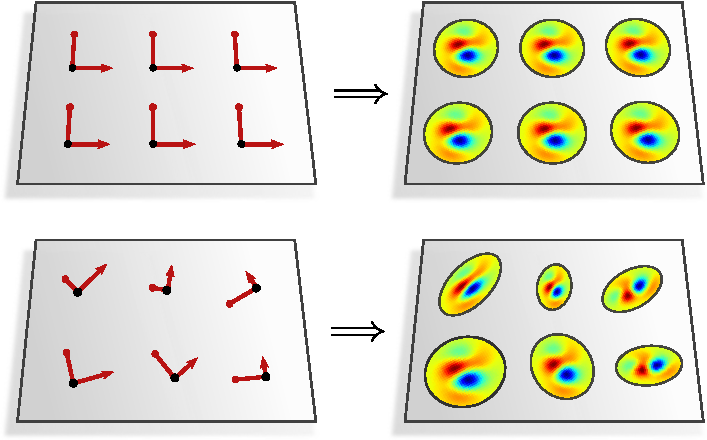
\includegraphics[width=.62\textwidth]{figures/intro_kernel_alignment_trivial.pdf}
	\captionsetup{width=.9\textwidth}
	\caption{\small
		خاصیت کلیدی کانولوشن‌ها این است که آنها وزن‌ها را روی منیفولد \emph{به اشتراک می‌گذارند}.
		ما تراز یک کرنل در \lr{$p\in M$} را با \emph{انتخاب چارچوب مرجع} -- یا \emph{گیج} -- فضای مماس متناظر~\lr{$\TpM$} شناسایی می‌کنیم.
		بنابراین \emph{میدان‌های چارچوب} مختلف \emph{میدان‌های کرنل} (کانولوشن) متفاوتی را دربر می‌گیرند.
		\\[1ex]
		انتخاب چارچوب‌ها اغلب یکتا نیست.
		ابهام در این انتخاب توسط \emph{ساختارهای} \lr{$G$} رسمی می‌شود؛ شکل~\ref{fig:G_structures_intro} را ببینید.
		برای در نظر گیری اختیاری بودن چارچوب‌ها، کرنل‌ها سپس نیاز دارند که قابل هدایت \lr{$G$} (هم‌متغیر) باشند همان‌طور که در شکل‌های~\ref{fig:intro_steerable_kernel} و~\ref{fig:intro_kernel_alignment_reflect} تجسم شده است.
		\\[0pt]
	}
	\label{fig:intro_kernel_alignment_trivial}
\end{SCfigure}





\subsubsection{ساختارهای \lr{\textit{G}}}
\label{sec:visual_intro_GM_subsub}

فضای \emph{تمام} چارچوب‌های ممکن \lr{$\TpM$} به عنوان~\lr{$\FpM$} نشان داده می‌شود.
\marginnote{بسته چارچوب \lr{$\FM$}}
در کنار هم، چارچوب‌های تمام فضاهای مماس \emph{بسته چارچوب}~\lr{$\FM$} را تشکیل می‌دهند؛ شکل~\ref{fig:frame_bundle} را ببینید.
هیچ انتخاب خاصی از چارچوب‌ها در \lr{$\FM$} روی منیفولد هموار «برهنه» (بدون ساختار هندسی بیشتر) نسبت به یکدیگر ترجیح داده نمی‌شود، که تراز کرنل‌ها را حداکثر مبهم می‌گذارد.
برای رفع ابهام چارچوب‌ها و تراز کرنل‌ها، منیفولد باید به \emph{ساختار هندسی اضافی} مجهز شود.


یک منیفولد ریمانی به \emph{ساختار متریک} مجهز است.
\marginnote{ساختار متریک \lr{$\OM$}}
با فراهم کردن ضرب داخلی (متریک ریمانی) روی فضاهای مماس، این ساختار امکان جدا کردن آن چارچوب‌های خاص که محورهایشان نسبت به یکدیگر \emph{متعامد نرمال} هستند را فراهم می‌کند.
\emph{تبدیل‌های گیج}، یعنی تبدیل‌ها بین انتخاب‌های چارچوب‌های مرجع (شکل‌های~\ref{fig:intro_gauge_isom_induction} (چپ) و~\ref{fig:gauge_trafos} را ببینید)، سپس مقادیری در \emph{گروه متعامد}~\lr{$\O{d}$} می‌گیرند.
روی منیفولدهای ریمانی تراز کرنل‌ها بنابراین همواره تا چرخش‌ها و انعکاس‌ها رفع ابهام می‌شود.


\lr{CNN}های اقلیدسی کرنل‌های کانولوشن (و بنابراین چارچوب‌ها) را
\marginnote{ساختارهای \lr{$G$} به نام \lr{$\GM$}}
موازی با یکدیگر تراز می‌کنند همان‌طور که در شکل~\ref{fig:intro_kernel_alignment_trivial} (بالا) تجسم شده است.
\lr{CNN}های کروی تراز کرنل‌ها را معمولاً تا چرخش‌ها رفع ابهام می‌کنند، یعنی آنها دست‌چینی ترجیحی چارچوب‌های مرجع را فرض می‌کنند.
ساختار متریک به تنهایی برای توصیف این تنظیمات ناکافی است، که نشان می‌دهد این منیفولدها به \emph{ساختار هندسی بیشتری علاوه بر ساختار متریک} مجهز هستند.
ما پیشنهاد می‌کنیم که چارچوب ریاضی مناسب، چارچوب \emph{ساختارهای} \lr{$G$} است و فرض می‌کنیم:

\begin{minipage}{\textwidth}
	\begin{center}\it
		ابهام در انتخاب چارچوب‌های مرجع (و بنابراین تراز کرنل‌ها) \\
		روی منیفولد \lr{$M$} توسط ساختار \lr{$G$} آن به نام \lr{$\GM$} رسمی می‌شود.
	\end{center}
\end{minipage}

ساختارهای \lr{$G$} به نام \lr{$\GM$} \emph{بسته‌هایی از چارچوب‌های مرجع متمایز} روی \lr{$M$} هستند به طوری که \emph{تبدیل‌های گیج} بین چارچوب‌های همان فضای مماس مقادیری در \emph{گروه ساختار}~\lr{${G\leq\GL{d}}$} می‌گیرند.
به طور شهودی، می‌توان در مورد مجموعه \lr{$\GpM$} چارچوب‌های \lr{$\TpM$} به عنوان «شبیه به» \lr{$G$} فکر کرد، با این حال، بدون مبدأ متمایز.%
\footnote{
	\lr{$\GpM$} یک \emph{فضای همگن اصلی} از~\lr{$G$} (یا \lr{$G$}-تورسور) است.
}


بسته چارچوب \lr{$\FM$} خودش یک ساختار \lr{$G$} با~\lr{${G=\GL{d}}$} است، در حالی که بسته چارچوب‌های متعامد نرمال \lr{$\OM$} یک ساختار \lr{$G$} (ساختار متریک) با~\lr{${G=\O{d}}$} است.
\lr{CNN}های اقلیدسی مرسوم بر میدان چارچوب متعارف روی \lr{$\R^d$} نشان داده شده در شکل~\ref{fig:G_structure_intro_a} تکیه می‌کنند، که یک ساختار \lr{$G$} برای گروه بدیهی~\lr{${G=\{e\}}$} است.
شکل~\ref{fig:G_structures_intro} ساختارهای \lr{$G$} را برای منیفولدها و گروه‌های ساختار بیشتر تجسم می‌کند.
مروری بر گروه‌های ساختار رایج در جدول~\ref{tab:G_structures} در بخش~\ref{sec:local_G-structure_G-atlas} یافت می‌شود.


ما در ادامه همواره فرض می‌کنیم که منیفولدهای ریمانی علاوه بر ساختار متریک خود به ساختار \lr{$G$} اضافی مجهز هستند.%
\footnote{
	ساختار \lr{$G$} باید با ساختار متریک سازگار باشد به این معنی که چارچوب‌های متمایز در \lr{$\GM$} زیرمجموعه‌ای از چارچوب‌های متعامد نرمال در \lr{$\OM$} هستند وقتی \lr{$G<\O{d}$}.
	به طور خاص برای \lr{$G=\O{d}$}، ساختار \lr{$G$} به نام \lr{$\GM$} با ساختار متریک \lr{$\OM$} منطبق است و هیچ اطلاعات هندسی اضافی اضافه نمی‌کند.
}
انتخاب خاص ساختار \lr{$G$} خواص شبکه عصبی را تعیین می‌کند؛ ما در بخش~\ref{sec:intro_overview_G_structure_choice} در زیر در مورد این انتخاب نظر خواهیم داد.





%%%%%%%%%%%%%%%%%%%%%%%%%%%%%%%%%%%%%%%%%%%%%%%%%%%%%%%%%%%%%%%%%%%%%%%%%%%%%%%%%%%%%%%%%%%%%%%%%%%%%%%%%%
\afterpage{ % execute argument of this command *after* end of current page
	\clearpage % clear any pending floats
	%%%%%%%%%%%%%%%%%%%%%%%%%%%%%%%%%%%%%%%%%%%%%%%%%%%%%%%%%%%%%%%%%%%%%%%%%%%%%%%%%%%%%%%%%%%%%%%%%%%%%%%%%%
	\begin{figure}
		\centering
		\vspace*{-4.ex}
		\begin{subfigure}[b]{0.26\textwidth}
	\centering
	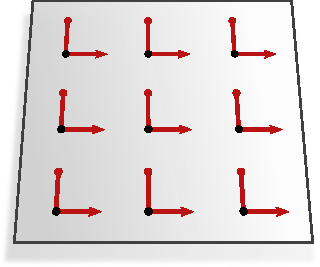
\includegraphics[width=1.\textwidth]{figures/G_structure_R2_1_big.pdf}
	\captionsetup{format=hang}
	\caption{\small
		\,$M = \R^2$,
		\,$G = \{e\}$
	}
	\label{fig:G_structure_intro_a}
\end{subfigure}
\hfill
\begin{subfigure}[b]{0.26\textwidth}
	\centering
	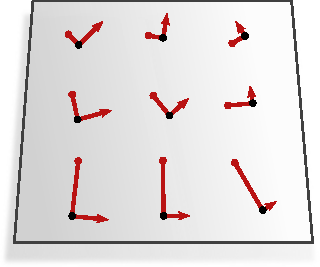
\includegraphics[width=1.\textwidth]{figures/G_structure_R2_5_big.pdf}
	\captionsetup{format=hang}
	\caption{\small
		\,$M = \R^2$,
		\,$G = \{e\}$
	}
	\label{fig:G_structure_intro_b}
\end{subfigure}
\hfill
\begin{subfigure}[b]{0.26\textwidth}
	\centering
	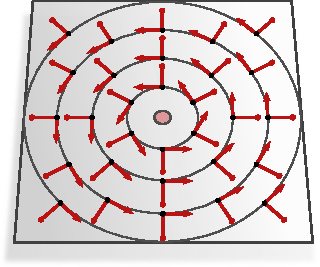
\includegraphics[width=1.\textwidth]{figures/G_structure_R2_no_origin_SO2_intro.pdf}
	\captionsetup{format=hang}
	\caption{\small
		\,$M = \R^2\backslash\{0\}$,
		\,$G = \{e\}$
	}
	\label{fig:G_structure_intro_c}
\end{subfigure}
\\[2ex]
%
%
%
%
\begin{subfigure}[b]{0.26\textwidth}
	\centering
	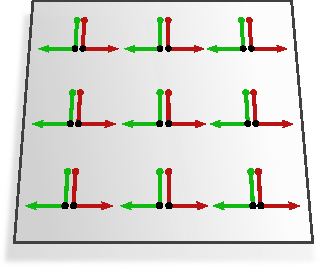
\includegraphics[width=1.\textwidth]{figures/G_structure_R2_3_big.pdf}
	\captionsetup{format=hang}
	\caption{\small
		\,$M = \R^2$,
		\,$G = \Flip$
	}
	\label{fig:G_structure_intro_d}
\end{subfigure}
\hfill
\begin{subfigure}[b]{0.26\textwidth}
	\centering
	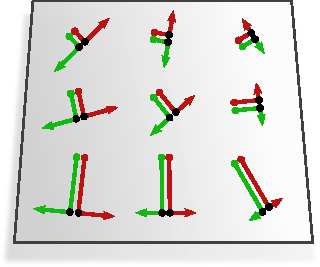
\includegraphics[width=1.\textwidth]{figures/G_structure_R2_6_big.pdf}
	\captionsetup{format=hang}
	\caption{\small
		\,$M = \R^2$,
		\,$G = \Flip$
	}
	\label{fig:G_structure_intro_e}
\end{subfigure}
\hfill
\begin{subfigure}[b]{0.26\textwidth}
	\centering
	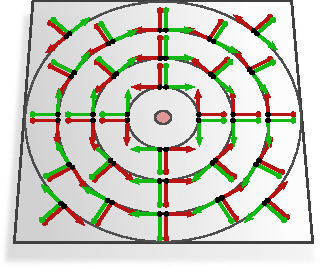
\includegraphics[width=1.\textwidth]{figures/G_structure_R2_no_origin_O2_intro.pdf}
	\captionsetup{format=hang}
	\caption{\small
		\,$M = \R^2\backslash\{0\}$,
		\,$G = \Flip$
	}
	\label{fig:G_structure_intro_f}
\end{subfigure}
\\[2ex]
%
%
%
%
\begin{subfigure}[b]{0.26\textwidth}
	\centering
	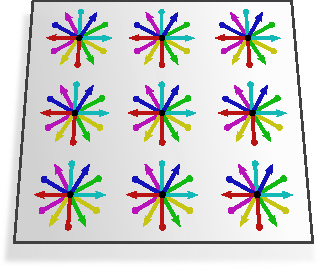
\includegraphics[width=1.\textwidth]{figures/G_structure_R2_2_big.pdf}
	\captionsetup{format=hang}
	\caption{\small
		\,$M = \R^2$,
		\,$G = \SO2$
	}
	\label{fig:G_structure_intro_g}
\end{subfigure}
\hfill
\begin{subfigure}[b]{0.26\textwidth}
	\centering
	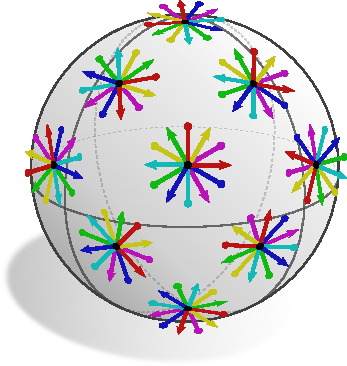
\includegraphics[width=.95\textwidth]{figures/G_structure_S2_1.pdf}
	\vspace*{-2ex}
	\captionsetup{format=hang}
	\caption{\small
		\,$M = S^2$,
		\,$G = \SO2$
	}
	\label{fig:G_structure_intro_h}
\end{subfigure}
\hfill
\begin{subfigure}[b]{0.26\textwidth}
	\centering
	\makebox[\textwidth][c]{ % center over-wide figure
		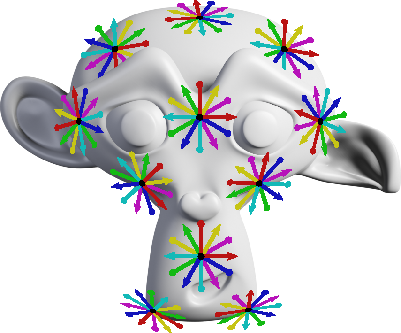
\includegraphics[width=1.12\textwidth]{figures/suzanne_SO2_structure.pdf}
	}
	\vspace*{-3.ex}
	\captionsetup{format=hang, width=1.1\textwidth}
	\caption{\small
		$M = \textup{``\href{https://en.wikipedia.org/wiki/Blender_(software)\#Suzanne}{\lr{Suzanne}}''}$\!,
		\ $G = \SO2$
	}
	\label{fig:G_structure_intro_i}
\end{subfigure}
\\[2ex]
%
%
%
%
\begin{subfigure}[b]{0.26\textwidth}
	\centering
	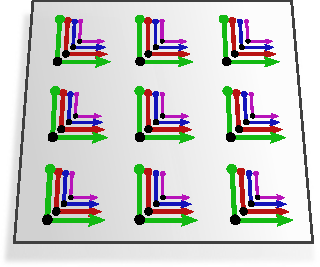
\includegraphics[width=1.\textwidth]{figures/G_structure_R2_4_big.pdf}
	\captionsetup{format=hang}
	\caption{\small
		\,$M = \R^2$,
		\,$G = \Scale$
	}
	\label{fig:G_structure_intro_j}
\end{subfigure}
\hfill
\begin{subfigure}[b]{0.26\textwidth}
	\centering
	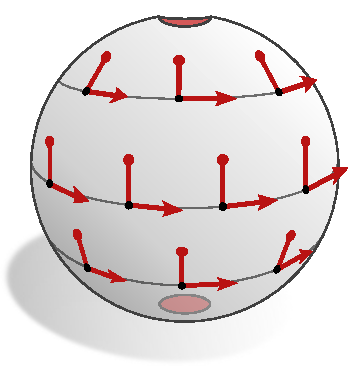
\includegraphics[width=.95\textwidth]{figures/G_structure_S2_2.pdf}
	\vspace*{-2ex}
	\captionsetup{format=hang}
	\caption{\small
		\,$M = S^2\backslash\text{\lr{poles}}$,
		\,$G = \{e\}$
	}
	\label{fig:G_structure_intro_k}
\end{subfigure}
\hfill
\begin{subfigure}[b]{0.26\textwidth}
	\centering
	\makebox[\textwidth][c]{ % center over-wide figure
		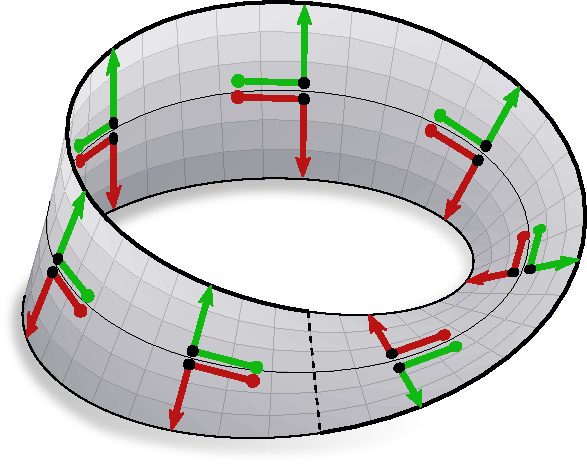
\includegraphics[width=1.1\textwidth]{figures/Mobius_R_structure.pdf}
	}
	\vspace*{-3.ex}
	\captionsetup{format=hang}
	\caption{\small
		\,$M = \textup{\lr{M\"obius}}$,
		\,$G = \Flip$
	}
	\label{fig:G_structure_intro_l}
\end{subfigure}
		\vspace*{1.5ex}
		\captionsetup{width=1.1\textwidth}
		\caption{\small
			نمونه‌هایی از ساختارهای \lr{$G$} به نام \lr{$\GM$} برای گروه‌های ساختار \lr{$G$} مختلف و روی منیفولدهای \lr{$M$} متفاوت.
			گروه ساختار \lr{$G$} نشان می‌دهد که تبدیل‌های گیج چه مقادیری می‌توانند بگیرند، و بنابراین زیرمجموعه چارچوب‌های متمایز در هر نقطه~\lr{$p$} چقدر «بزرگ» است.
			شکل~\ref{fig:G_structure_intro_a} ساختار متعارف \lr{$\{e\}$} (میدان چارچوب) \lr{$\R^2$} را نشان می‌دهد که مطابق با \lr{CNN}های اقلیدسی مرسوم است.
			\mbox{ساختارهای \lr{$G$}} در
			شکل‌های~\ref{fig:G_structure_intro_d}، \ref{fig:G_structure_intro_g} و~\ref{fig:G_structure_intro_j}
			با اضافه کردن چارچوب‌های منعکس (\lr{$G=\Flip$})، چرخیده (\lr{$G=\SO2$}) و مقیاس‌بندی شده (\lr{$G=\Scale$}) به ترتیب ساخته می‌شوند.
			کانولوشن‌های \lr{$\GM$} متناظر نه تنها هم‌متغیر انتقال بلکه هم‌متغیر تحت عمل گروه‌های آفین~\lr{$\Aff(G)$} هستند.
			\mbox{ساختارهای \lr{$G$}} معمولاً یکتا نیستند.
			شکل‌های~\ref{fig:G_structure_intro_b} و~\ref{fig:G_structure_intro_e} ساختارهای \lr{$G$} جایگزین روی~\lr{$\R^2$} را نشان می‌دهند (مطابق با متریک جایگزین که نسبت به آن چارچوب‌هایشان متعامد نرمال هستند).
			آنها ممکن است از لحاظ عملی مرتبط نباشند اما انعطاف‌پذیری چارچوب ما را نشان می‌دهند.
			ساختار \lr{$\{e\}$} در شکل~\ref{fig:G_structure_intro_c} مطابق با مختصات قطبی است.
			از آنجا که ساختارهای \lr{$G$} باید پیوسته باشند، ما مبدأ~\lr{0} را که مختصات قطبی در آن تکین است، حذف کردیم.
			می‌توان بار دیگر ساختار \lr{$\Flip$} را با اضافه کردن چارچوب‌های منعکس همان‌طور که در شکل~\ref{fig:G_structure_intro_f} نشان داده شده، تعریف کرد.
			این ساختارهای \lr{$G$} کانولوشن‌هایی روی \lr{$\R^2\backslash\{0\}$} را مدل می‌کنند که \lr{$\SO2$} و \lr{$\O2$}-هم‌متغیر هستند اما هم‌متغیر انتقال نیستند.
			شکل~\ref{fig:G_structure_intro_h} ساختار معمول \lr{$\SO2$} روی ۲-کره نهفته~\lr{$S^2$} را نشان می‌دهد که زیربنای \lr{CNN}های کروی \lr{$\SO3$}-هم‌متغیر است.
			انتخاب محبوب دیگر ساختار \lr{$\{e\}$} در شکل~\ref{fig:G_structure_intro_k} است که توسط مختصات کروی القا می‌شود.
			توجه کنید که این ساختار \lr{$\{e\}$} در قطب‌ها تکین خواهد بود که بنابراین بریده می‌شوند.
			کاهش‌های پیوسته (یعنی غیرتکین) گروه ساختار فراتر از~\lr{$\SO2$} روی کره از لحاظ توپولوژیکی مسدود هستند.
			بنابراین کرنل‌های قابل هدایت \lr{$G$} با \lr{$G\geq\SO2$} به طور کامل برای کانولوشن‌های پیوسته روی کره‌های توپولوژیکی مانند مِش در شکل~\ref{fig:G_structure_intro_i} ضروری هستند.
			شکل~\ref{fig:G_structure_intro_l} ساختار \lr{$\Flip$} روی نوار موبیوس را نشان می‌دهد.
			از آنجا که نوار موبیوس غیرقابل جهت‌یابی است، کاهش پیوسته گروه ساختار فراتر از گروه انعکاس~\lr{$G=\Flip$} را نمی‌پذیرد.
		}
		\label{fig:G_structures_intro}
	\end{figure}
	%%%%%%%%%%%%%%%%%%%%%%%%%%%%%%%%%%%%%%%%%%%%%%%%%%%%%%%%%%%%%%%%%%%%%%%%%%%%%%%%%%%%%%%%%%%%%%%%%%%%%%%%%%
	\thispagestyle{empty}
	\clearpage % force a page break
}
%%%%%%%%%%%%%%%%%%%%%%%%%%%%%%%%%%%%%%%%%%%%%%%%%%%%%%%%%%%%%%%%%%%%%%%%%%%%%%%%%%%%%%%%%%%%%%%%%%%%%%%%%%


\subsubsection{شبکه‌های مستقل از مختصات \lr{\textit{GM}}}
هدف ما
\marginnote{استقلال از مختصات \lr{$\GM$} (کوواریانس)}
طراحی شبکه‌های عصبی روی منیفولدهای ریمانی با ساختار اضافی \lr{$G$} است.
اگر گروه ساختار \lr{$G$} غیر بدیهی باشد، \emph{هیچ انتخاب متعارف برای چارچوب‌های مرجع (گیج) وجود ندارد} طبق تعریف.
با این حال، برای انجام محاسبات عددی، \emph{برخی} گیج، که نسبت به آن کرنل‌ها و ویژگی‌ها بیان می‌شوند، باید انتخاب شود.
از آنجا که این انتخاب ذاتاً اختیاری است، ما تقاضا می‌کنیم که استنتاج شبکه‌ها در نهایت به آن وابسته نباشد، یعنی ما نیاز داریم:
\begin{center}\it
	شبکه‌های عصبی روی منیفولد ریمانی با ساختار \lr{$G$} به نام \lr{$\GM$} \\
	باید بر پایه عملیات «مستقل از مختصات \lr{$\GM$}» باشند.
\end{center}
«استقلال از مختصات \lr{$\GM$}» به این معنی است که \emph{تمام کمیت‌های هندسی و توابع بین آنها باید به طور مساوی در هر گیجی قابل بیان باشند}، یعنی نسبت به هر انتخابی از چارچوب‌های مرجع ساختار \lr{$G$}.
مورد خاص ضرایب بردار مماس و تبدیل‌های گیج بین آنها در شکل~\ref{fig:gauge_trafos} نمایش داده شده است.
شکل~\ref{sec:gauges_TpM_functions} نمونه‌ای از نگاشت خطی و نمایش مستقل از مختصات آن در قالب ماتریس‌های نسبت به چارچوب‌های مختلف را نشان می‌دهد.


توجه کنید که نیاز به استقلال از مختصات \lr{$\GM$} کاملاً انعطاف‌پذیر است:
برای \lr{$G=\GL{d}$} داریم \lr{$\GM=\FM$} و بنابراین حداکثر سطح استقلال از مختصات.
در انتهای دیگر طیف گروه‌های ساختار، \lr{$G=\{e\}$} داریم که برای آن \lr{$\GM$} یک میدان چارچوب ثابت است و استقلال از مختصات \lr{$\GM$} به وابستگی صریح مختصات تقلیل می‌یابد.
آزادی انتخاب ساختارهای \lr{$G$} اختیاری امکان کنترل دقیق استقلال از مختصات شبکه‌ها را فراهم می‌کند،
که در عمل به طور گسترده متفاوت است؛ برای مثال جدول~\ref{tab:network_instantiations} در بخش~\ref{part:literature_review} را ببینید.


شبکه‌های ما \emph{میدان‌های بردار ویژگی} روی منیفولد را پردازش می‌کنند.
\marginnote{میدان‌های بردار ویژگی مرتبط با \lr{$G$}}
بردارهای ویژگی کمیت‌های هندسی \emph{مستقل از مختصات} هستند مانند مثلاً بردارهای مماس.
نسبت به چارچوب انتخابی (گیج) ممکن است توسط \emph{بردارهای ضریب عددی} نمایش داده شوند.
تقاضا برای استقلال از مختصات \lr{$\GM$} نیاز دارد که ضرایب عددی در گیج‌های مختلف همان محتوای اطلاعاتی را کدگذاری کنند.
این امر به طور طبیعی با مرتبط کردن ویژگی‌ها با نمایش گروهی~\lr{$\rho$} از گروه ساختار~\lr{$G$} که رفتار تبدیل ضرایب آنها را تحت تبدیل‌های گیج تعیین می‌کند، حاصل می‌شود:
\begin{center}\it
	میدان‌های بردار ویژگی با نمایش \lr{$G$} به نام \lr{$\rho$} مرتبط هستند که \\
	قانون تبدیل ضرایب عددی آنها را هنگام تبدیل بین چارچوب‌های مرجع مشخص می‌کند.
	\\[1ex]
	از لحاظ فنی، میدان‌های ویژگی بخش‌هایی از بسته‌های بردار ویژگی مرتبط با \lr{$G$} هستند.
\end{center}
نمونه‌های معمول شامل میدان‌های اسکالر، میدان‌های بردار مماس یا سایر میدان‌های تانسوری هستند، اما هر قانون تبدیلی قابل قبول است و می‌تواند توسط کاربر انتخاب شود.
سایر انتخاب‌های رایج برای~\lr{$\rho$} در زمینه یادگیری عمیق شامل نمایش‌های غیرقابل تقلیل یا منظم است؛
نمونه‌های بیشتر در جدول~\ref{tab:network_instantiations} در بخش~\ref{part:literature_review} فهرست شده‌اند.


ما می‌خواهیم تأکید کنیم که نیاز به استقلال از مختصات \lr{$\GM$} صرفاً یک \emph{شرط سازگاری} است که تضمین می‌کند ناظران مختلف (چارچوب‌ها) روی همان مشاهده هندسی مستقل از مختصات توافق دارند.
این امر مجموعه توابع قابل قبول را به هیچ وجه محدود \emph{نمی‌کند}، بلکه تنها نحوه ارتباط بیان‌های آنها نسبت به چارچوب‌های مختلف را مشخص می‌کند.
به طور خاص، \emph{شبکه‌های عصبی مستقل از مختصات \lr{$\GM$} به طور کلی مجبور به هم‌متغیر گیج بودن نیستند}.
نیاز به هم‌متغیری گیج زمانی پیروی می‌کند که همزمان تقاضای اشتراک وزن و استقلال از مختصات شود، یعنی کانولوشن‌های مستقل از مختصات \lr{$\GM$} بر کرنل‌های هم‌متغیر گیج تکیه می‌کنند.



\begin{SCfigure}[2.5]
	\centering
	\small
	\begin{tabular}{c@{\hspace{2pt}}c}
		\rotatebox{-90}{
			\includegraphicstotab[width=.12\textwidth]{figures/kernels/K_symmetric.png}
		} &
		\reflectbox{\rotatebox{-90}{
				\includegraphicstotab[width=.12\textwidth]{figures/kernels/K_antisymmetric.png}
		}} \\[60pt]
		اسکالر & اسکالر \\
		$\updownarrow$ & $\updownarrow$ \\
		اسکالر & شبه‌اسکالر
	\end{tabular}
	\hspace*{-2.5ex}
	\caption[]{\small
		کرنل‌های قابل هدایت \lr{$G$} نمونه برای گروه \lr{$G=\mathrm{Flip}$} انعکاس‌ها در امتداد محور اول چارچوب (تبدیل‌های پاریته).
		محدودیت‌های هم‌متغیری کرنل‌ها به انواع میدان \lr{$\rho_{\mathrm{in}}$} و \lr{$\rho_{\mathrm{out}}$} ورودی و خروجی کانولوشن بستگی دارد.
		میدان‌های اسکالر و شبه‌اسکالر توسط نمایش بدیهی و نمایش تغییر علامت \lr{$\mathrm{Flip}$} به ترتیب توصیف می‌شوند.
		کرنل‌های قابل هدایت که بین چنین میدان‌هایی نگاشت می‌کنند محدود به متقارن یا نامتقارن بودن هستند.
		\\[1ex]
		توجه کنید که کرنل‌های قابل هدایت به طور کلی مقدار اسکالر ندارند بلکه مقدار ماتریس \lr{$c_{\mathrm{out}} \times c_{\mathrm{in}}$} دارند، جایی که \lr{$c_{\mathrm{out}}$} و \lr{$c_{\mathrm{in}}$} ابعاد بردارهای ویژگی خروجی و ورودی به ترتیب هستند.
		اشتقاق و نمونه‌های بیشتر برای سایر انواع میدان (ابعاد بالاتر) \lr{$G=\mathrm{Flip}$} در بخش~\ref{sec:mobius_kernel_spaces} و جدول~\ref{tab:reflection_steerable_kernels} یافت می‌شود.
		کرنل‌های قابل هدایت برای \lr{$G=\mathrm{SO}(2)$} یا \lr{$G=\mathrm{SO}(3)$} از هارمونیک‌های دایره‌ای \cite{Weiler2019_E2CNN,Worrall2017-HNET,Weiler2018SFCNN} یا کروی \cite{3d_steerableCNNs,Thomas2018-TFN} ساخته می‌شوند.
		اگر~\lr{$G$} فشرده باشد، کرنل‌های قابل هدایت \lr{$G$} توسط تعمیمی از قضیه ویگنر-اکارت~\cite{lang2020WignerEckart} توصیف می‌شوند.
		\\[-20pt]
	}
	\label{fig:intro_steerable_kernel}
\end{SCfigure}


\subsubsection{کانولوشن‌های مستقل از مختصات \lr{\textit{GM}}}
ما به سؤال اولیه خود بازمی‌گردیم
\marginnote{اشتراک وزن مستقل از مختصات \lr{$\GM$} $~\mkern22mu~\Longleftrightarrow$ قابلیت هدایت \lr{$G$}}
در مورد اینکه چگونه یک کرنل کانولوشن را به اشتراک بگذاریم با توجه به اینکه تراز آن ذاتاً مبهم است وقتی گروه ساختار~\lr{$G$} غیر بدیهی است.
از آنجا که عملیات کانولوشن باید مستقل از مختصات \lr{$\GM$} باشد، روش اشتراک وزن زیربنایی نیز باید مستقل از انتخاب‌های اختیاری چارچوب‌های مرجع باشد.
تراز کرنل در امتداد چارچوب‌های مختلف ساختار \lr{$G$} در نقطه‌ای~\lr{$p$} بنابراین همواره باید نتایج معادلی به دست دهد.
ما نشان می‌دهیم که استقلال از مختصات \lr{$\GM$} فرآیند اشتراک وزن محدودیت \emph{هم‌متغیری گیج} («قابلیت هدایت \lr{$G$}») را بر کرنل‌های کانولوشن تحمیل می‌کند:


\begin{center}
	\begin{tabular}{r@{}}
		استقلال از مختصات \lr{$\mathcal{G}M$} \\[4pt]
		اشتراک وزن
	\end{tabular}
	$\Bigg\} \longrightarrow$ قابلیت هدایت \lr{$G$} (هم‌متغیری گیج)
\end{center}
شکل~\ref{fig:intro_steerable_kernel} و جدول~\ref{tab:reflection_steerable_kernels} نمونه‌هایی از کرنل‌های قابل هدایت انعکاس را نشان می‌دهند.
محدودیت هم‌متغیری (قابلیت هدایت) نوعی از تقارن \lr{$G$} را اعمال می‌کند که تضمین می‌کند \emph{پاسخ‌های کرنل به طور قابل پیش‌بینی} تحت تبدیل‌های گیج تبدیل شوند.
یک نمایش بصری از اینکه چگونه کرنل‌های قابل هدایت \lr{$G$} ابهام چارچوب‌های مرجع را حل می‌کنند در شکل~\ref{fig:intro_kernel_alignment_reflect} ارائه شده است.


%%%%%%%%%%%%%%%%%%%%%%%%%%%%%%%%%%%%%%%%%%%%%%%%%%%%%%%%%%%%%%%%%%%%%%%%%%%%%%%%%%%%%%%%%%%%%%%%%%%%%%%%%%%%%%%%%%%%%%%%%
\begin{samepage}
	کانولوشن‌های مستقل از مختصات \lr{$\GM$} (یا به اختصار کانولوشن‌های \lr{$\GM$})
	{\setlength{\marginparwidth}{2.5cm}% prevent marginnote from moving to next line when being too wide
		\marginnote{کانولوشن‌های \lr{$\GM$}}}%
	به عنوان کانولوشن‌هایی با کرنل‌های قابل هدایت \lr{$G$} تعریف می‌شوند:
	\begin{center}\it
		یک کانولوشن \lr{$\GM$} با کرنل قابل هدایت \lr{$G$} به نام \lr{$K$} ویژگی‌ها را با اعمال این \\
		کرنل در هر نقطه \lr{$p\in M$} نسبت به انتخاب اختیاری چارچوب مرجع در \lr{$\GpM$} پردازش می‌کند. \\
	\end{center}
\end{samepage}
%%%%%%%%%%%%%%%%%%%%%%%%%%%%%%%%%%%%%%%%%%%%%%%%%%%%%%%%%%%%%%%%%%%%%%%%%%%%%%%%%%%%%%%%%%%%%%%%%%%%%%%%%%%%%%%%%%%%%%%%%
اختیاری بودن گیج انتخابی بدین ترتیب توسط قابلیت هدایت \lr{$G$} کرنل تضمین می‌شود.
در حالی که در مختصات محلی ساخته می‌شوند، 
کانولوشن‌های \lr{$\GM$} مطابق با عملیات کانولوشن \emph{مستقل از مختصات} به خوبی تعریف شده روی منیفولد هستند.


نه تنها کرنل‌های کانولوشن بلکه \emph{هر تابع قالب مشترک نیاز به هم‌متغیر گیج بودن دارد} تا استقلال از مختصات \lr{$\GM$} را حفظ کند.
بخش~\ref{sec:pointwise_operations} محدودیت‌های هم‌متغیری روی بایاس‌های مشترک، کرنل‌های \onexone\ و غیرخطی‌ها را مشتق می‌کند.
توجه کنید که محدودیت‌های هم‌متغیری روی توابع قالب مشترک می‌توانند به عنوان شکلی از اشتراک وزن روی چارچوب‌های مرجع مرتبط با \lr{$G$} در نظر گرفته شوند
-- ابهام اشتراک وزن روی منیفولد~\lr{$M$} بنابراین با گسترش اشتراک وزن روی کل ساختار \lr{$G$} به نام~\lr{$\GM$} حل می‌شود.



\begin{figure}
	\centering
	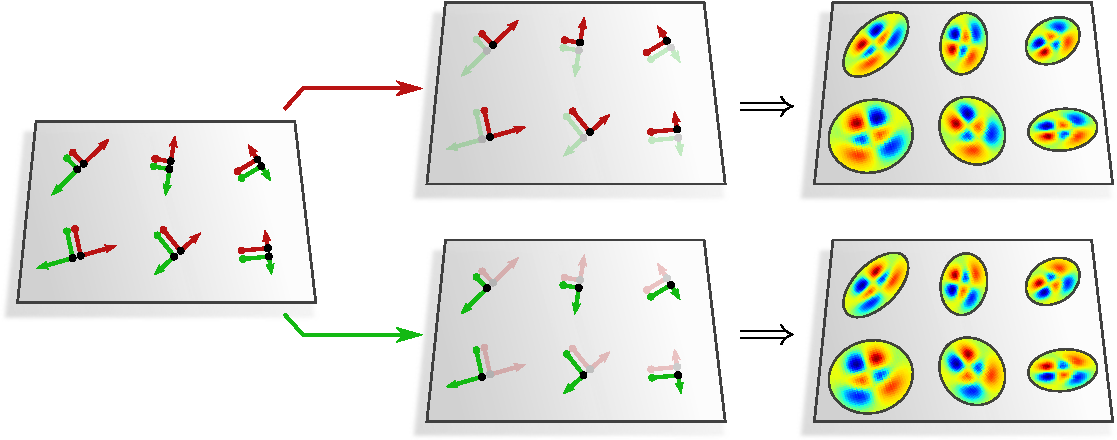
\includegraphics[width=1.\textwidth]{figures/intro_kernel_alignment_reflect.pdf}
	\caption{\small
		اشتراک یک کرنل قابل هدایت \lr{$\Flip$} بر اساس ساختار \lr{$\Flip$} داده شده به نام \lr{$\RM$} روی منیفولد~\lr{$M = \R^2$}.
		دو گیج پیوسته (قرمز و سبز) وجود دارد که کرنل می‌تواند در امتداد آنها به اشتراک گذاشته شود.
		به دلیل هم‌متغیری \lr{$\Flip$} آن، انتخاب خاص در نهایت بی‌ربط است.
		کرنل تجسم شده نامتقارن است و بنابراین بین میدان‌های اسکالر و شبه‌اسکالر نگاشت می‌کند.
		به راحتی می‌توان تأیید کرد که واقعاً چنین است:
		ضرایب عددی یک میدان ورودی اسکالر تحت تبدیل‌های گیج ثابت باقی می‌مانند اما کرنل‌ها منعکس می‌شوند.
		از آنجا که آنها نامتقارن هستند، پاسخ‌هایشان منفی خواهد شد -- که قانون تبدیل ضرایب عددی یک میدان شبه‌اسکالر است.
		استدلال مشابهی برای نگاشت‌ها از شبه‌اسکالرها به اسکالرها برقرار است.
		چگونه می‌توانستیم از اسکالرها به اسکالرها نگاشت کنیم؟
		در این مورد هم ورودی و هم خروجی باید ثابت گیج باشند، که نیاز دارد کرنل به جای نامتقارن، متقارن باشد.
		کرنل‌های متقارن علاوه بر این بین میدان‌های شبه‌اسکالر نگاشت می‌کنند.
	}
	\label{fig:intro_kernel_alignment_reflect}
\end{figure}




\toclesslab\subsection{هم‌متغیری تحت تقارن‌های سراسری منیفولد}{sec:intro_overview_isometry}

\begin{SCfigure}
	\centering
	\hspace*{2ex}
	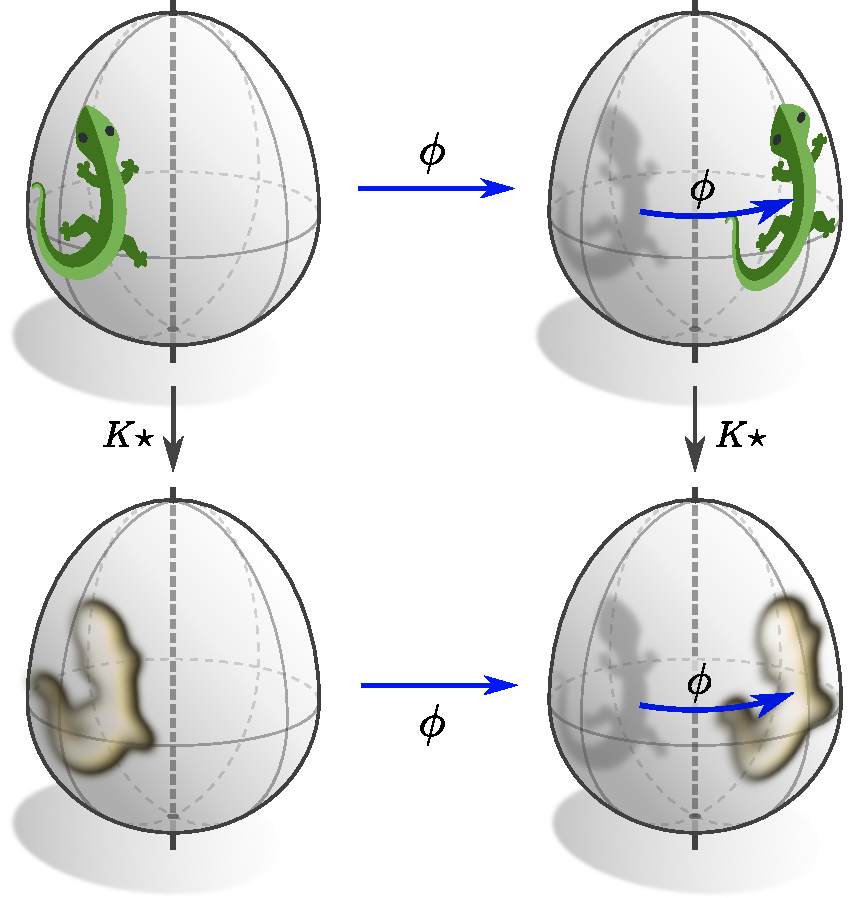
\includegraphics[width=.5\textwidth]{figures/lizard_conv_egg_intro.pdf}
	\captionsetup{width=.9\textwidth}
	\caption[]{\small
		تجسم یک کانولوشن \lr{$\GM$} هم‌متغیر ایزومتری.
		یک ایزومتری \lr{$\phi$} از طریق انتقال به جلو روی میدان‌های ویژگی عمل می‌کند.
		کانولوشن \lr{$\GM$} به نام \lr{$K\star$} با کرنل قابل هدایت \lr{$G$} به نام \lr{$K$} هم‌متغیر نسبت به این ایزومتری گفته می‌شود وقتی پاسخ کانولوشن یک ورودی تبدیل شده (\lr{$\rightarrow,\downarrow$}) با انتقال به جلو پاسخ ورودی تبدیل نشده (\lr{$\downarrow,\rightarrow$}) موافق باشد.
		\\[1ex]
		کانولوشن‌های \lr{$\GM$} نسبت به (زیر)گروه \lr{$\mathrm{Isom}_{\mathcal{G}M}$} ایزومتری‌هایی که تقارن‌های ساختار \lr{$G$} هستند، هم‌متغیر هستند.
		هم‌متغیری چرخش آزیموتال تجسم شده بنابراین نیاز به ساختار \lr{$G$} دارد که تحت چرخش‌ها حول محور قطبی ثابت باشد -- این شرط برای مثال توسط مشابه ساختارهای \lr{$G$} کروی در شکل‌های~\ref{fig:G_structure_intro_h} و~\ref{fig:G_structure_intro_k} روی تخم‌مرغ برآورده می‌شود.
		گروه ایزومتری منیفولد تخم‌مرغی‌شکل نه تنها شامل چرخش‌ها بلکه انعکاس‌ها نیز هست.
		برای دستیابی به هم‌متغیری انعکاس، ساختارهای \lr{$G$} علاوه بر این باید شامل چارچوب‌های منعکس باشند و کانولوشن \lr{$\GM$} باید کرنل‌های قابل هدایت انعکاس اعمال کند.
		{\\
			\color{gray}
			\scriptsize
			(مارمولک‌ها تحت مجوز \lr{Creative Commons Attribution 4.0 International}
			\href{https://github.com/twitter/twemoji/blob/gh-pages/LICENSE-GRAPHICS}{\underline{اقتباس شده}}
			با تشکر از \lr{Twitter}.)
		}
		\\[-16pt]
	}
	\label{fig:lizard_conv_egg_intro}
\end{SCfigure}


عملیات کانولوشن اغلب طراحی می‌شوند تا نسبت به تقارن‌های فضای زیربنایی هم‌متغیر باشند \cite{Cohen2016-GCNN,Kondor2018-GENERAL}.
تقارن‌های یک منیفولد ریمانی گروه \emph{ایزومتری} آن به نام \lr{$\mathrm{Isom}(M)$} را تشکیل می‌دهند، که گروه تمام نگاشت‌های حافظ فاصله~\lr{${\phi:M\to M}$} است.
ایزومتری‌ها به طور طبیعی روی کمیت‌های هندسی مانند بردارهای ویژگی با «حرکت دادن آنها همراه با» عمل ایزومتری (انتقال به جلو) عمل می‌کنند؛ شکل~\ref{fig:intro_gauge_isom_induction} (وسط) را ببینید.
علی‌رغم اینکه تنها برای هم‌متغیر بودن تحت تبدیل‌های گیج محلی طراحی شده‌اند،
کانولوشن‌های \lr{$\GM$} نسبت به عمل زیرگروه‌های ایزومتری خاص \lr{$\mathrm{Isom}_{\mathcal{G}M} \leq \mathrm{Isom}(M)$} روی میدان‌های ویژگی هم‌متغیر هستند.
این زیرگروه‌ها \lr{$\mathrm{Isom}_{\mathcal{G}M}$} شامل آن \emph{ایزومتری‌هایی هستند که تقارن‌های ساختار \lr{$G$} محسوب می‌شوند}.
طراحی کانولوشن‌های \lr{$\GM$} هم‌متغیر ایزومتری بنابراین با طراحی ساختارهای \lr{$G$} ثابت مرتبط است.
شکل~\ref{fig:lizard_conv_egg_intro} ایده یک کانولوشن \lr{$\GM$} هم‌متغیر ایزومتری را به طور گرافیکی تجسم می‌کند.


ما در ادامه به طور مختصر محدودیت‌های تقارن که نیاز به هم‌متغیری ایزومتری بر میدان‌های کرنل، یعنی بر اتصال عصبی، تحمیل می‌کند را بحث خواهیم کرد.
این شرایط روی میدان‌های کرنل مطابق با محدودیت‌های تقارن روی ساختارهای \lr{$G$} است که کرنل‌های کانولوشن در امتداد آنها به اشتراک گذاشته می‌شوند.
در نهایت در مورد اینکه چرا کانولوشن‌های \lr{$\GM$} تنها هم‌متغیر ایزومتری هستند و به طور کلی نسبت به دیفئومورفیسم‌های عمومی‌تر هم‌متغیر نیستند، نظر خواهیم داد.






\pagebreak






\subsubsection{میدان‌های کرنل ثابت ایزومتری}
\label{sec:visual_intro_inv_kernel_fields}

خواص هم‌متغیری یک شبکه عصبی
\marginnote{تبدیل‌های میدان کرنل}
در نهایت به تقارن‌ها در اتصال عصبی آن بستگی دارد~\cite{ravanbakhsh2017EquivarianceParameterSharing}.
برای شبکه‌های کانولوشن این امر معادل \emph{محدودیت‌های تقارن روی میدان کرنل} است.
برای مطالعه این محدودیت‌ها در کلیت کامل، ما نیاز نداریم که میدان‌های کرنل \emph{کانولوشن} باشند، یعنی توسط یک کرنل مشترک واحد تعیین شوند،
بلکه \emph{میدان‌های کرنل عمومی} را فرض می‌کنیم که ممکن است کرنل متفاوتی در هر نقطه از فضا اعمال کنند.
ما لایه‌های شبکه متناظر را به عنوان \emph{«تبدیل‌های میدان کرنل»} نشان می‌دهیم:%
\footnote{
	تبدیل‌های میدان کرنل در ادبیات بینایی کامپیوتر گاهی «\emph{شبکه‌های متصل محلی}» نامیده می‌شوند.
}
\begin{center}\it
	«تبدیل‌های میدان کرنل» شبیه کانولوشن‌های \lr{$\GM$} هستند اما ممکن است کرنل متفاوتی در هر نقطه اعمال کنند. \\
	بنابراین آنها توسط میدان‌های کرنل عمومی پارامتری می‌شوند.
\end{center}
کانولوشن‌های \lr{$\GM$} تبدیل‌های میدان کرنل خاصی با میدان‌های کرنل کانولوشن \lr{$\GM$} هستند.
نتایج کلی برای تبدیل‌های میدان کرنل هم‌متغیر ایزومتری بنابراین فوراً به کانولوشن‌های \lr{$\GM$} تعمیم می‌یابند.


قضیه~\ref{thm:isometry_equivariant_kernel_field_trafos} ثابت می‌کند
\marginnote{میدان‌های کرنل ثابت ایزومتری}
که تناوب یک میدان کرنل تحت عمل ایزومتری و هم‌متغیری تبدیل میدان کرنل متناظر یکدیگر را نتیجه می‌دهند:
\begin{center}\it
	میدان کرنل ثابت ایزومتری
	$\quad \Longleftrightarrow \quad$
	تبدیل میدان کرنل هم‌متغیر ایزومتری
\end{center}
میدان‌های کرنل ثابت به دو روش کیفیتاً متفاوت محدود می‌شوند:
اولاً، کرنل‌ها باید روی \emph{مدارهای ایزومتری} به اشتراک گذاشته شوند.
ثانیاً، کرنل‌های مشترک خود توسط \emph{زیرگروه تثبیت‌کننده} مدار متناظر محدود می‌شوند.
توجه کنید که میدان کرنل کامل و متقارن می‌تواند از یک کرنل نماینده واحد برای هر مدار بازیابی شود --
قضیه‌های~\ref{thm:tangent_quotient_repr_kernel_fields} و~\ref{thm:manifold_quotient_repr_kernel_fields} این گزاره را با اثبات یکریختی‌هایی بین میدان‌های کرنل ثابت روی منیفولد و میدان‌های کرنل روی فضاهای خارج‌قسمت تحت عمل ایزومتری رسمی می‌کنند.

\begin{figure}
	\hspace{1.ex}
	\begin{subfigure}[b]{0.24\textwidth}
		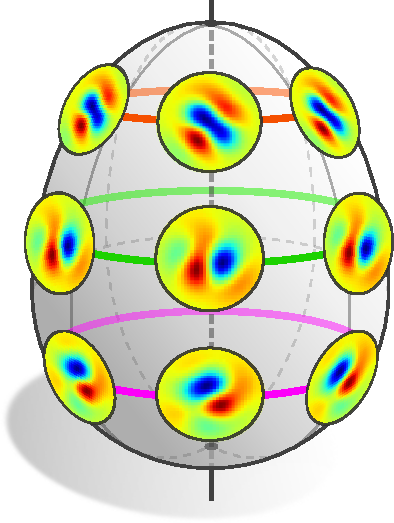
\includegraphics[width=.92\textwidth]{figures/isometry_egg_intro_symmetric.pdf}
		\vspace*{-.5ex}
		\captionsetup{format=hang, width=.7\textwidth}
		\caption{\small
			میدان کرنل ثابت \lr{$\mathrm{SO}(2)$}
		}
		\label{fig:isom_invariant_kernel_field_intro_SO2}
	\end{subfigure}
	\hspace*{1.5ex}
	\begin{subfigure}[b]{0.24\textwidth}
		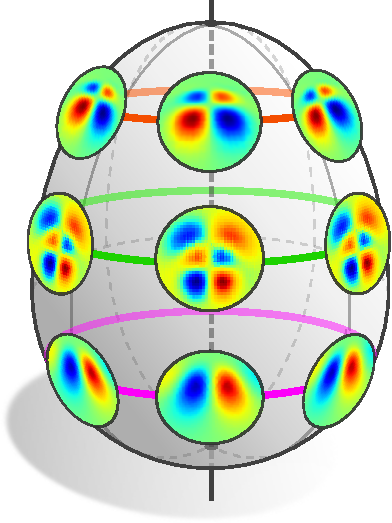
\includegraphics[width=.92\textwidth]{figures/isometry_egg_intro_antisymmetric.pdf}
		\vspace*{-.5ex}
		\captionsetup{format=hang, width=.7\textwidth}
		\caption{\small
			میدان کرنل ثابت \lr{$\mathrm{O}(2)$}
		}
		\label{fig:isom_invariant_kernel_field_intro_O2}
	\end{subfigure}
	\par
	\vspace*{\dimexpr-\parskip-158.pt\relax}% Skip backwards over last left-aligned image
	\parshape 17 % Set flow of caption: N lines...
	.55\textwidth .45\textwidth % First N-1 start @ .55\textwidth with a width of .45\textwidth
	.55\textwidth .45\textwidth
	.55\textwidth .45\textwidth
	.55\textwidth .45\textwidth
	.55\textwidth .45\textwidth
	.55\textwidth .45\textwidth
	.55\textwidth .45\textwidth
	.55\textwidth .45\textwidth
	.55\textwidth .45\textwidth
	.55\textwidth .45\textwidth
	.55\textwidth .45\textwidth
	.55\textwidth .45\textwidth
	.55\textwidth .45\textwidth
	.55\textwidth .45\textwidth
	.55\textwidth .45\textwidth
	.55\textwidth .45\textwidth
	.01\textwidth .98\textwidth % the last (N-th) line flows from 0 to .99 = .62+.37 = .01+.98 ad infinitum
	\makeatletter
	\setcounter{\@captype}{\value{\@captype}-1} % \setcounter{CounterName}{number}
	\refstepcounter{\@captype}% Increase float/caption counter
	\addcontentsline{\csname ext@\@captype\endcsname}{\@captype}% Add content to "List of..."
	{\protect\numberline{\csname the\@captype\endcsname}{ToC entry}}%
	\small % switch to small font for caption and Figure XX:
	\csname fnum@\@captype\endcsname: % Float caption + #
	\makeatother
	\hyphenpenalty = 300 % default should be 50, however, without setting this parameter no hyphens occurred
	% Actual caption
	\emph{تبدیل‌های میدان کرنل} شبیه کانولوشن‌های \lr{$\GM$} هستند اما ممکن است کرنل متفاوتی در هر نقطه اعمال کنند.
	قضیه~\ref{thm:isometry_equivariant_kernel_field_trafos} ثابت می‌کند که \emph{تبدیل‌های میدان کرنل هم‌متغیر ایزومتری} در تناظر یک به یک با \emph{میدان‌های کرنل ثابت ایزومتری} هستند.
	این امر شامل
	۱) اشتراک وزن روی \emph{مدارهای ایزومتری} (حلقه‌های رنگی) و
	۲) محدودیت روی کرنل‌ها برای قابل هدایت بودن نسبت به \emph{زیرگروه تثبیت‌کننده} مدار مربوطه‌شان است.
	شکل~\ref{fig:isom_invariant_kernel_field_intro_SO2} میدان کرنل ثابت \lr{$\mathrm{SO}(2)$} روی منیفولد تخم‌مرغی‌شکل را نشان می‌دهد.
	مدارهای مختلف آزادند که کرنل‌های متفاوت را بدون به خطر انداختن هم‌متغیری \lr{$\mathrm{SO}(2)$} استفاده کنند.
	کرنل‌ها خود محدود نیستند چون زیرگروه‌های تثبیت‌کننده عمل \lr{$\mathrm{SO}(2)$} روی مدارها بدیهی هستند (به جز در قطب‌ها).
	شکل~\ref{fig:isom_invariant_kernel_field_intro_O2} مورد میدان کرنل ثابت \lr{$\mathrm{O}(2)$} را تجسم می‌کند.
	مدارها یکسان هستند، با این حال، زیرگروه‌های تثبیت‌کننده محدودیت هم‌متغیری انعکاسی تحمیل می‌کنند.
	توجه کنید که مفهوم تناوب به عمل گروه روی کرنل، تعریف~\ref{dfn:isometry_action_kernel_fields}، بستگی دارد که به نوبه خود به نمایش‌های میدان ویژگی انتخاب شده وابسته است.
	کرنل‌های نامتقارن به این معنی تحت انعکاس‌ها ثابت هستند.
	\label{fig:isom_invariant_kernel_field_intro}
\end{figure}


شکل‌های~\ref{fig:isom_invariant_kernel_field_intro_SO2} و~\ref{fig:isom_invariant_kernel_field_intro_O2}
\marginnote{نمونه‌ها}
این نتایج را برای منیفولد تخم‌مرغی‌شکل که ایزومتری‌هایش چرخش‌ها و انعکاس‌ها حول محور عمودی هستند، نمونه می‌زنند.
یک تبدیل میدان کرنل عمومی می‌تواند هر میدان کرنلی اعمال کند.
اگر تنها هم‌متغیری ایزومتری \lr{$\mathrm{SO}(2)$} نیاز باشد (بدون انعکاس‌ها)، مدارها حلقه‌هایی حول تخم‌مرغ هستند و زیرگروه تثبیت‌کننده عمل \lr{$\mathrm{SO}(2)$} روی این مدارها بدیهی است؛ شکل~\ref{fig:isom_invariant_kernel_field_intro_SO2} را ببینید.%
\footnote{
	ما برای اختصار قطب‌ها را نادیده می‌گیریم، جایی که زیرگروه تثبیت‌کننده در شکل~\ref{fig:isom_invariant_kernel_field_intro_SO2} برابر \lr{$\mathrm{SO}(2)$} و در شکل~\ref{fig:isom_invariant_kernel_field_intro_O2} برابر \lr{$\mathrm{O}(2)$} است.
}
میدان کرنل ثابت ایزومتری بنابراین کرنل‌های بدون محدودیت را روی این مدارها به اشتراک می‌گذارد.
شکل~\ref{fig:isom_invariant_kernel_field_intro_O2} میدان کرنل ثابت \lr{$\mathrm{O}(2)$} را نشان می‌دهد.
مدارها، و بنابراین الگوی اشتراک وزن فضایی، در اینجا همانند مورد قبلی هستند.
با این حال، زیرگروه تثبیت‌کننده عمل \lr{$\mathrm{O}(2)$} روی مدارها گروه انعکاس است.
کرنل‌ها بنابراین محدود به قابل هدایت انعکاس بودن هستند، با محدودیت دقیق بسته به انواع \lr{$\rho_{\mathrm{in}}$} و \lr{$\rho_{\mathrm{out}}$} میدان ویژگی ورودی و خروجی.


مورد جالب خاص
\marginnote{فضاهای همگن}
منیفولدهایی است که \emph{فضاهای همگن} گروه ایزومتری‌شان هستند.
در این مورد تنها یک مدار واحد وجود دارد، به طوری که میدان کرنل ثابت توسط \emph{یک کرنل مشترک (کانولوشن) واحد} تعیین می‌شود.
قضیه~\ref{thm:GM_conv_homogeneous_equivalence} ثابت می‌کند:
\begin{center}\it
	تبدیل‌های میدان کرنل هم‌متغیر ایزومتری روی فضاهای همگن لزوماً کانولوشن هستند.
\end{center}
کرنل‌ها بار دیگر نیاز دارند که نسبت به زیرگروه تثبیت‌کننده عمل ایزومتری قابل هدایت باشند.
این امر نتایج \citet{Kondor2018-GENERAL}، \citet{Cohen2019-generaltheory} و \citet{bekkers2020bspline} را بازیابی می‌کند که \lr{CNN}های هم‌متغیر گروه روی فضاهای همگن را بررسی کردند؛ پیوست~\ref{apx:homogeneous_conv} را برای مقایسه عمیق ببینید.


\subsubsection{هم‌متغیری ایزومتری کانولوشن‌های \lr{\textit{GM}}}
\label{sec:visual_intro_isom_equiv_conv}

\paragraph{ساختارهای \lr{\textit{G}} ثابت ایزومتری:}
کانولوشن‌های \lr{$\GM$} تبدیل‌های میدان کرنل خاصی هستند
\marginnote{ساختارهای \lr{$G$} ثابت ایزومتری}
که بر میدان‌های کرنل کانولوشن \lr{$\GM$} تکیه می‌کنند.
بنابراین آنها هم‌متغیر ایزومتری هستند اگر میدان کرنل کانولوشن \lr{$\GM$} تحت عمل ایزومتری ثابت باشد.
به یاد بیاورید که میدان‌های کرنل کانولوشن \lr{$\GM$} با اشتراک گذاری برخی کرنل قابل هدایت \lr{$G$} در امتداد چارچوب‌های (اختیاری) ساختار \lr{$G$} تعریف می‌شوند.
تقارن‌های آنها (ایزومتری‌ها) بنابراین با تقارن‌های ساختار \lr{$G$} منطبق هستند.
\begin{center}\it
	ما \lr{$\mathrm{Isom}_{\mathcal{G}M} \leq \mathrm{Isom}(M)$} را به عنوان زیرگروه آن ایزومتری‌هایی تعریف می‌کنیم که \\
	تقارن‌های ساختار \lr{$G$} به نام \lr{$\GM$} هستند (خودریختی‌های بسته اصلی).
\end{center}
\begin{minipage}{\textwidth}
	از این رو نتیجه می‌شود که
	\begin{center}\it
		میدان‌های کرنل کانولوشن \lr{$\GM$} ثابت \lr{$\mathrm{Isom}_{\mathcal{G}M}$} هستند.
	\end{center}
	\vspace*{1ex}\end{minipage}
\begin{minipage}{\textwidth}
	در نتیجه، که در قضیه~\ref{thm:isom_equiv_GM_conv} به طور دقیق اثبات شده، می‌یابیم:
	\begin{center}\it
		کانولوشن‌های \lr{$\GM$} هم‌متغیر \lr{$\mathrm{Isom}_{\mathcal{G}M}$} هستند.
	\end{center}
	\vspace*{1ex}\end{minipage}
طراحی کانولوشن‌های \lr{$\GM$} هم‌متغیر ایزومتری بنابراین به طراحی ساختارهای \lr{$G$} ثابت ایزومتری تقلیل می‌یابد.
شکل~\ref{fig:intro_invariant_kernel_fields_plane} دو نمونه از ساختارهای \lr{$G$} به نام \lr{$\GM$} و میدان‌های کرنل کانولوشن \lr{$\GM$} متناظر را نشان می‌دهد که همان تقارن‌ها را به اشتراک می‌گذارند.
برای نمونه‌های بیشتر به ساختارهای \lr{$G$} در شکل~\ref{fig:G_structures_intro} مراجعه می‌کنیم.
توجه کنید که \lr{$\mathrm{Isom}_{\mathcal{G}M}$} برای \lr{$G=\mathrm{O}(d)$} (یا ابرگروه‌های آن) شامل تمام ایزومتری‌های ممکن است، که نتیجه می‌دهد کانولوشن‌های \lr{$\GM$} متناظر کاملاً \lr{$\mathrm{Isom}(M)$}-هم‌متغیر هستند.
گزاره مشابهی برای \lr{$G=\mathrm{SO}(d)$} و ایزومتری‌های حافظ جهت‌یابی برقرار است.

\begin{SCfigure}
	\centering
	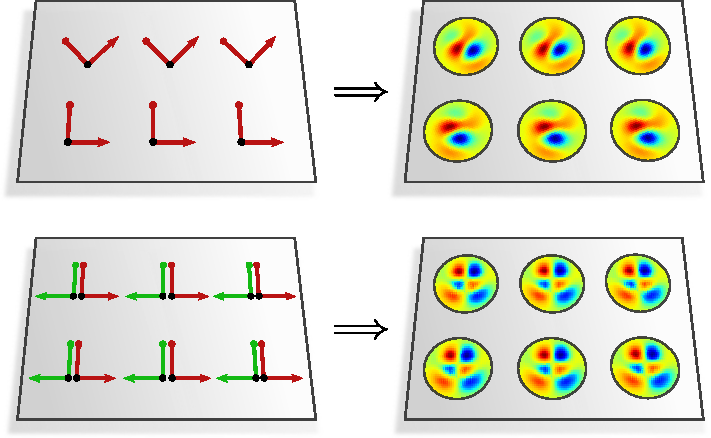
\includegraphics[width=.62\textwidth]{figures/intro_invariant_kernel_fields_plane.pdf}
	\captionsetup{width=.92\textwidth}
	\caption{\small
		میدان‌های کرنل کانولوشن \mbox{\lr{$\GM$}} با اشتراک گذاری برخی کرنل قابل هدایت \lr{$G$} در امتداد چارچوب‌های (اختیاری) \mbox{ساختار \lr{$G$}} به نام \lr{$\GM$} ساخته می‌شوند.
		تقارن‌های میدان‌های کرنل بنابراین با تقارن‌های ساختار \lr{$G$}، یعنی با \lr{$\mathrm{Isom}_{\mathcal{G}M}$}، موافق هستند.
		ساختار \lr{$\{e\}$} که در بالا تجسم شده بنابراین مطابق با \mbox{کانولوشن \lr{$\GM$}} است که نسبت به انتقال‌ها در جهت افقی هم‌متغیر است اما در جهت عمودی نیست.
		از آنجا که \mbox{ساختار \lr{$\mathrm{Flip}$}} که در پایین تجسم شده تحت انتقال‌های اختیاری و انعکاس‌های افقی ثابت است، \mbox{کانولوشن \lr{$\GM$}} ضمنی هم‌متغیر انتقال و انعکاس است.
		\\[-5pt]
	}
	\label{fig:intro_invariant_kernel_fields_plane}
\end{SCfigure}






\paragraph{تبدیل‌های گیج القا شده توسط ایزومتری:}

استدلال بر حسب میدان‌های کرنل ثابت
\marginnote{تبدیل‌های گیج القا شده توسط ایزومتری}
و ساختارهای \lr{$G$} ثابت بر هیچ انتخاب گیجی تکیه نمی‌کرد بلکه در تنظیم کاملاً هندسی و \emph{مستقل از مختصات} فرمول‌بندی شده بود.
نقطه نظر جایگزین هم‌متغیری ایزومتری کانولوشن‌های \lr{$\GM$} را در مختصات توضیح می‌دهد، جایی که ایزومتری‌ها از طریق تبدیل‌های گیج القا شده عمل می‌کنند.
این تبدیل‌های گیج توسط قابلیت هدایت \lr{$G$} کرنل توضیح داده می‌شوند، که پیوندی بین مفاهیم \emph{هم‌متغیری گیج} و \emph{هم‌متغیری ایزومتری} فراهم می‌کند.
ما در ادامه به طور مختصر این نقطه نظر جایگزین را شرح می‌دهیم.


وقتی \emph{نسبت به چارچوب‌های مرجع محلی} بیان می‌شوند، ایزومتری‌ها می‌توانند به عنوان عمل از طریق \emph{تبدیل‌های گیج القا شده} روی ضرایب بردار ویژگی در نظر گرفته شوند.
شکل~\ref{fig:intro_gauge_isom_induction} (راست) این مفهوم را تجسم می‌کند:
فرض کنید که چارچوب‌های مرجع را در نقطه‌ای \lr{$p$} و در تصویرش \lr{$\phi(p)$} تحت عمل ایزومتری~\lr{$\phi$} انتخاب کرده‌ایم.
ایزومتری یک ویژگی را از \lr{$p$} به \lr{$\phi(p)$} هل می‌دهد.
از آنجا که هندسه‌های ریمانی حول \lr{$p$} و \lr{$\phi(p)$} غیرقابل تشخیص هستند، تنها چیزی که از نقطه نظر بردار ویژگی تغییر کرده نسبت به کدام چارچوب مرجع بیان می‌شود.
این تغییر چارچوب‌ها تبدیل گیج القا شده توسط ایزومتری است.

\begin{figure}
	\centering
	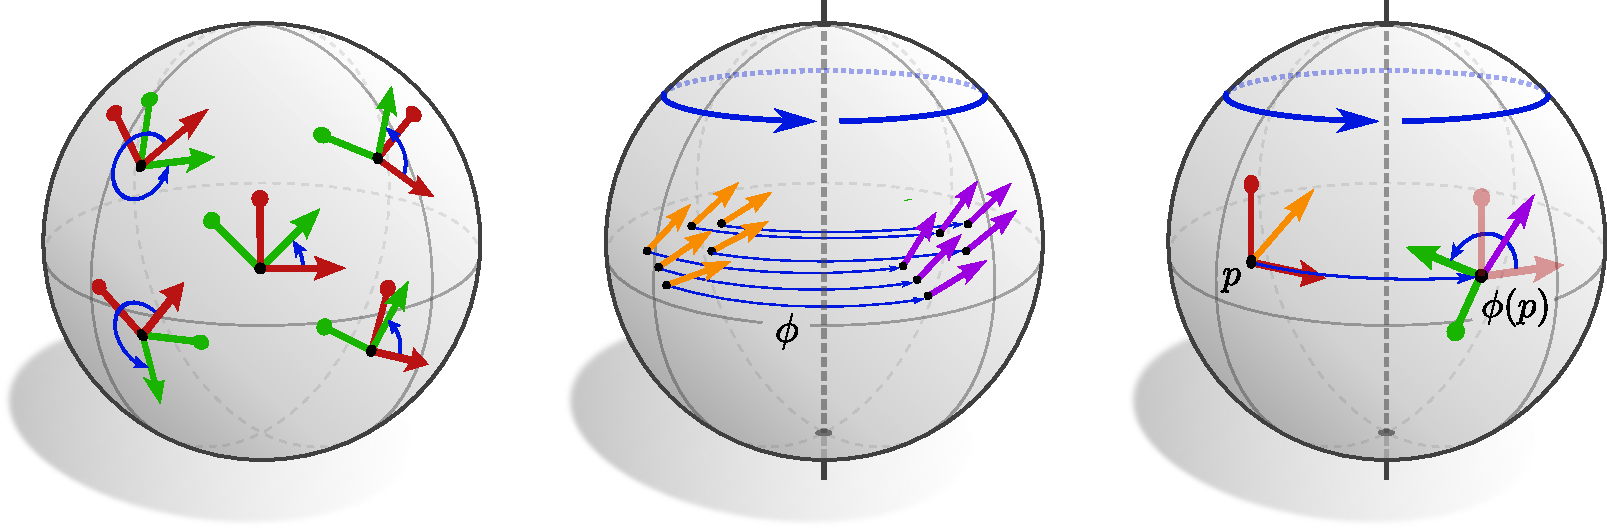
\includegraphics[width=.98\columnwidth]{figures/intro_gauge_isom_equiv.pdf}
	\vspace*{-1ex}
	\caption{\small
		تبدیل‌های گیج، ایزومتری‌ها و رابطه متقابل آنها.
		\ \ \emph{چپ:}
		گیج انتخاب چارچوب‌های مرجع محلی (میدان چارچوب) است که نسبت به آن کمیت‌های هندسی ممکن است بیان شوند.
		اگر گروه ساختار منیفولد \lr{$G$} غیر بدیهی باشد، انتخاب گیج یکتا نیست بلکه انتخاب‌های معادل زیادی وجود دارد.
		انتخاب‌های مختلف گیج‌ها (قرمز یا سبز) توسط تبدیل‌های گیج (آبی) مرتبط هستند که طبق تعریف مقادیری در گروه ساختار~\lr{$G$} می‌گیرند.
		چارچوب‌های متعامد نرمال راست‌گرد تجسم شده‌اند که برای آنها تبدیل‌های گیج مقدار \lr{$G=\mathrm{SO}(2)$} دارند.
		\ \ \emph{وسط:}
		ایزومتری‌ها تقارن‌های منیفولدهای ریمانی هستند.
		آنها به عنوان توابع حافظ فاصله \lr{$\phi: M \to M$} تعریف می‌شوند که منیفولد را به خودش نگاشت می‌کنند.
		ایزومتری‌ها از طریق انتقال به جلو روی بردارهای مماس، چارچوب‌های مرجع و بردارهای ویژگی عمل می‌کنند.
		در حالی که تبدیل‌های گیج تبدیل‌های مختصات غیرفعال هستند، ایزومتری‌ها به طور فعال نقاط و کمیت‌های هندسی را روی منیفولد حرکت می‌دهند.
		\ \ \emph{راست:}
		وقتی نسبت به چارچوب‌های مرجع محلی بیان می‌شوند، عمل ایزومتری‌ها می‌تواند به عنوان القای تبدیل‌های گیج در نظر گرفته شود.
		فرض کنید چارچوب‌ها در \lr{$p$} (قرمز) و \lr{$\phi(p)$} (سبز) داده شده باشند.
		یک کمیت هندسی در \lr{$p$} (نارنجی) توسط ایزومتری به \lr{$\phi(p)$} (بنفش) هل داده می‌شود.
		از آنجا که \lr{$\phi$} ایزومتری است، هندسه ریمانی حول \lr{$p$} و \lr{$\phi(p)$} غیرقابل تشخیص است، با این حال، انتقال به جلو کمیت هندسی نسبت به چارچوب مرجع جدیدی (سبز به جای قرمز) بیان می‌شود.
		بنابراین می‌توان ایزومتری‌ها را به عنوان القاکننده تبدیل‌های گیج در نظر گرفت.
		اگر این تبدیل‌های گیج القا شده مقادیری در گروه ساختار \lr{$G$} بگیرند، توسط قابلیت هدایت \lr{$G$} (هم‌متغیری گیج) کرنل‌های کانولوشن توضیح داده می‌شوند -- کانولوشن‌های \lr{$\GM$} آنگاه هم‌متغیر ایزومتری هستند.
		این شرط همواره برای \lr{$G\geq\mathrm{O}(d)$} برآورده می‌شود.
	}
	\label{fig:intro_gauge_isom_induction}
\end{figure}


به یاد بیاورید که کانولوشن‌های \lr{$\GM$} همان کرنل قابل هدایت \lr{$G$} را در هر نقطه از منیفولد اعمال می‌کنند.
هم‌متغیری \lr{$G$} کرنل هر تبدیل گیج مقدار \lr{$G$} (القا شده) را در نظر می‌گیرد، به طوری که:
\begin{center}\it
	اگر ایزومتری تبدیل‌های گیجی القا کند که مقادیری در گروه ساختار~\lr{$G$} بگیرند، \\
	آنگاه هر کانولوشن \lr{$\GM$} نسبت به این ایزومتری هم‌متغیر است.
\end{center}


تبدیل‌های گیج القا شده برای ایزومتری‌های عمومی ممکن است مقادیری در گروه ساختار انتخابی~\lr{$G$} نگیرند.
برای مثال، ساختارهای \lr{$G$} در شکل‌های~\ref{fig:G_structure_intro_a} و~\ref{fig:G_structure_intro_d} گروه‌های ساختار \lr{$G=\{e\}$} و \lr{$G=\mathrm{Flip}$} به ترتیب دارند، اما چرخش‌های \lr{$M=\R^2$} تبدیل‌های گیج مقدار \lr{$\mathrm{SO}(2)$} یا \lr{$\mathrm{O}(2)$} القا می‌کنند.
با این حال، اگر ایزومتری تقارن ساختار \lr{$G$} باشد، یعنی عنصری از \lr{$\mathrm{Isom}_{\mathcal{G}M}$}، چارچوب‌ها در~\lr{$\GM$} را به چارچوب‌ها در~\lr{$\GM$} نگاشت می‌کند.
از آنجا که چارچوب‌ها در~\lr{$\GM$} توسط تبدیل‌های گیج مقدار \lr{$G$} مرتبط هستند، نتیجه می‌شود که:
\begin{center}\it
	ایزومتری‌ها در \lr{$\mathrm{Isom}_{\mathcal{G}M}$} تبدیل‌های گیجی القا می‌کنند که مقادیری در گروه ساختار \lr{$G$} می‌گیرند.
\end{center}
این نتیجه می‌دهد که کانولوشن‌های \lr{$\GM$} هم‌متغیر \lr{$\mathrm{Isom}_{\mathcal{G}M}$} هستند، همان‌طور که قبلاً در تنظیم مستقل از مختصات یافت شد.
در حالی که این نقطه نظر جایگزین از لحاظ هندسی کمتر شهودی است، نقش قابلیت هدایت \lr{$G$} کرنل‌ها در هم‌متغیری ایزومتری شبکه‌ها را تأکید می‌کند.




\subsubsection{دیفئومورفیسم‌ها، ایزومتری‌ها و تبدیل‌های آفین:}
\label{sec:visual_intro_diffeo_equiv}

اکثر استدلال‌ها در بندهای قبلی نه تنها برای ایزومتری‌ها، بلکه برای دیفئومورفیسم‌ها نیز برقرار خواهند بود.
این سؤال را مطرح می‌کند که آیا کانولوشن‌های \lr{$\GM$} نسبت به گروه‌های دیفئومورفیسم عمومی‌تر هم‌متغیر هستند.
در برخی تنظیمات واقعاً چنین است، با این حال، کانولوشن‌های \lr{$\GM$} به طور کلی (علاوه بر این) بر ساختار متریک منیفولدها تکیه می‌کنند که تنها توسط ایزومتری‌ها حفظ می‌شود.


در بالا، کانولوشن‌های \lr{$\GM$} را به عنوان «اعمال کرنل قابل هدایت \lr{$G$} نسبت به چارچوب‌های ساختار \lr{$G$}» توصیف کردیم.
دقیق‌تر، کرنل در \emph{مختصات نرمال ژئودزیکی} اعمال می‌شود.
این بدان معنی است که میدان ویژگی در هر نقطه \lr{$p\in M$} از طریق \emph{نگاشت نمایی ریمانی} \lr{$\exp_p$} به فضای مماس \lr{$\TpM$} بازکشیده می‌شود، جایی که با کرنل تطبیق داده می‌شود؛ شکل~\ref{fig:pullback_field_exp_TpM} را ببینید.
در حالی که میدان کرنل خود تحت آن دیفئومورفیسم‌ها \lr{$\mathrm{Diff}_{\mathcal{G}M}\leq\mathrm{Diff}(M)$} که تقارن‌های ساختار \lr{$G$} هستند ثابت خواهد بود، نگاشت نمایی صراحتاً به ساختار متریک بستگی دارد.
کانولوشن‌های \lr{$\GM$} با \emph{کرنل‌های گسترده فضایی} بنابراین به طور کلی تنها می‌توانند هم‌متغیر ایزومتری باشند.


هر لایه شبکه که وزن‌ها را به اشتراک می‌گذارد و بر ساختار متریک منیفولدها تکیه نمی‌کند می‌تواند هم‌متغیر دیفئومورفیسم باشد.
نمونه‌های مهم لایه‌های هم‌متغیر \lr{$\mathrm{Diff}_{\mathcal{G}M}$} شامل \emph{عملیات نقطه‌ای} مانند جمع بایاس، غیرخطی‌ها و \onexone است که در بخش~\ref{sec:pointwise_operations} معرفی می‌شوند.
باید امکان تعمیم نظریه ما به \emph{معادلات دیفرانسیل جزئی عصبی روی منیفولدهای هموار} وجود داشته باشد که تعامل‌های غیرمحلی کانولوشن‌های \lr{$\GM$} را با \emph{تعامل‌های محلی} بر حسب عملگرهای دیفرانسیل قابل هدایت \lr{$G$} قابل یادگیری جایگزین کنند.
توجه کنید که کانولوشن‌های \lr{$\GM$} در عمل اغلب از کرنل‌های پشتیبانی فشرده استفاده می‌کنند و بنابراین \emph{شبه‌محلی}~\cite{tomboulis2015nonlocal} هستند.
هم‌متغیری \lr{$\mathrm{Diff}_{\mathcal{G}M}$} چنین کانولوشن‌های \lr{$\GM$} با کرنل‌های کوچک باید تقریباً برقرار باشد.


مورد خاص کانولوشن‌های \lr{$\GM$} روی فضاهای اقلیدسی است.
نگاشت نمایی روی فضاهای اقلیدسی نه تنها توسط ایزومتری‌ها، بلکه توسط هر \emph{تبدیل آفین} حفظ می‌شود.
قضیه~\ref{thm:affine_equivariance_Euclidean_GM_conv} ثابت می‌کند که کانولوشن‌های \lr{$\GM$} اقلیدسی واقعاً تحت عمل گروه‌های آفین \lr{$\mathrm{Aff}(G)$} (معادله~\eqref{eq:AffG_def}) هم‌متغیر هستند اگر ساختارهای \lr{$G$} ثابت آفین مانند ستون اول شکل~\ref{fig:G_structures_intro} انتخاب شوند.
این شامل ایزومتری‌های \lr{$\mathrm{E}(d)$} فضاهای اقلیدسی، اما همچنین مثلاً \emph{\lr{CNN}های هم‌متغیر مقیاس} است.



















\toclesslab\subsection{در مورد انتخاب ساختارهای \lr{\textit{G}}}{sec:intro_overview_G_structure_choice}

\begin{SCfigure}
	\centering
	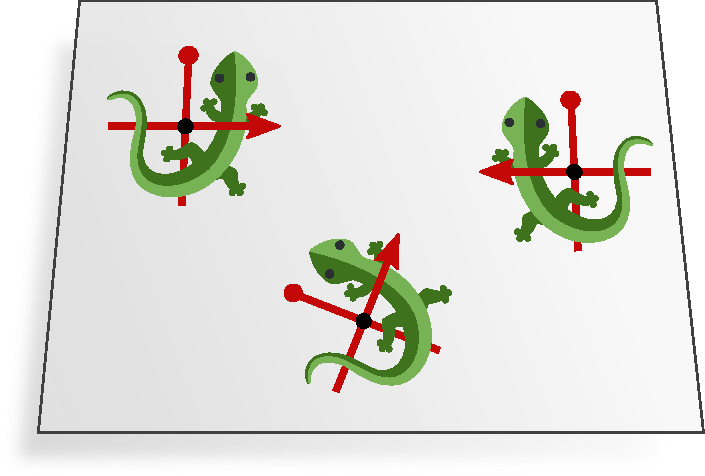
\includegraphics[width=.46\columnwidth]{figures/intro_lizard.pdf}
	\captionsetup{width=1\textwidth}
	\hspace{1.5ex}
	\caption{\small
		الگوهای معمول در سیگنال‌ها معمولاً در ژست‌های هندسی متفاوت ظاهر می‌شوند.
		کانولوشن‌های \lr{$\GM$} روی تمام ژست‌هایی که توسط عمل گروه ساختار انتخابی~\lr{$G$} مرتبط هستند تعمیم می‌دهند.
		در حالی که یک \lr{CNN} مرسوم روی \lr{${M=\R^2}$} باید یاد بگیرد تمام مارمولک‌ها را به طور جداگانه تشخیص دهد، یک \lr{CNN} مستقل از مختصات \lr{$\GM$} برای \lr{$G=\mathrm{SO}(2)$} بین مارمولک چپ و پایین تعمیم می‌دهد و برای \lr{$G=\mathrm{Flip}$} بین مارمولک چپ و راست تعمیم می‌دهد.
		برای \lr{$G=\mathrm{O}(2)$}، تضمین می‌شود که هر سه مارمولک را به عنوان \emph{همان ویژگی} در \emph{ژست‌های متفاوت} کدگذاری کند.
		{
			\color{gray}
			\scriptsize
			(مارمولک‌ها تحت مجوز \lr{Creative Commons Attribution 4.0 International}
			\href{https://github.com/twitter/twemoji/blob/gh-pages/LICENSE-GRAPHICS}{\underline{اقتباس شده}}
			با تشکر از \lr{Twitter}.)
		}
		\\\protect\rule{0ex}{2.5ex}
	}
	\label{fig:intro_lizard}
\end{SCfigure}


نکته‌ای که تاکنون باز گذاشته شده انتخاب ساختار \lr{$G$} است.
به طور کلی، یک منیفولد ریمانی با ساختار متریک، یعنی ساختار \lr{$\mathrm{O}(d)$} می‌آید.
کاهش گروه ساختار به زیرگروه‌های \lr{$G<\mathrm{O}(d)$} ممکن است توسط توپولوژی منیفولد مسدود شود
-- ساختارهای \lr{$G$} \emph{هموار} (یا پیوسته) \emph{وجود ندارند} اگر چنین باشد.
به جز از این محدودیت، انتخاب ساختار \lr{$G$} عمدتاً سؤال مهندسی است که برای مثال به خواص هم‌متغیری مطلوب بستگی دارد.


در اکثر کاربردها
\marginnote{موانع توپولوژیکی}
منطقی است که تقاضا کنیم پیش‌بینی شبکه عصبی به طور \emph{هموار} روی منیفولد تغییر کند.
از آنجا که کانولوشن‌های \lr{$\GM$} کرنل‌ها را نسبت به چارچوب‌های برخی ساختار \lr{$G$} به اشتراک می‌گذارند، پاسخ کانولوشن تنها زمانی تضمین می‌شود که هموار باشد که ساختار \lr{$G$} هموار باشد.
این واقعیت شناخته شده است که توپولوژی منیفولد کاهش (هموار) گروه ساختارش را فراتر از سطح خاصی مسدود می‌کند.
این نتیجه می‌دهد که \emph{حداقل سطحی از هم‌متغیری گیج کاملاً ضروری است} برای عملیات کانولوشن هموار.
ما در قضیه~\ref{thm:existence_kernel_field_trafo_compact_kernels} ثابت می‌کنیم که کانولوشن‌های \lr{$\GM$} ما واقعاً همواری میدان‌های ویژگی را حفظ می‌کنند.


نمونه شهودی از چنین مانع توپولوژیکی غیرقابل جهت‌یابی بودن نوار موبیوس از شکل~\ref{fig:G_structure_intro_l} است:
کاهش گروه ساختار به گروه بدیهی \lr{$\{e\}$} مطابق با انتخاب میدان چارچوب هموار روی نوار خواهد بود.
با این حال، به دلیل پیچش نوار، این کاهش لزوماً منجر به ناپیوستگی در قالب انعکاس چارچوب در نقطه‌ای خواهد شد
-- کاهش به \lr{$G=\{e\}$} بنابراین از لحاظ توپولوژیکی مسدود است و کرنل‌های قابل هدایت \lr{$\mathrm{Flip}$} روی نوار موبیوس اجتناب‌ناپذیر هستند.
نمونه دیگر ۲-کره~\lr{$S^2$} است که کاهش فراتر از~\lr{$G=\mathrm{SO}(2)$} را نمی‌پذیرد.


در ادبیات یادگیری عمیق غیرمعمول نیست
\marginnote{شبکه‌های ناپیوسته}
که چنین موانع توپولوژیکی نادیده گرفته شوند و شبکه‌های ناپیوسته پیاده‌سازی شوند.
نمونه‌ای \lr{CNN}های کروی هستند که بر ساختار \lr{$\{e\}$} در شکل~\ref{fig:G_structure_intro_k} تکیه می‌کنند؛ بخش~\ref{sec:spherical_CNNs_azimuthal_equivariant} را برای بررسی دقیق چنین مدل‌هایی ببینید.
توجه کنید که حذف قطب‌ها، جایی که میدان چارچوب تکین است، توپولوژی کروی را به توپولوژی استوانه‌ای تبدیل می‌کند، جایی که کاهش هموار به \lr{$G=\{e\}$} امکان‌پذیر است.
بخش~\ref{sec:e_surface_conv} کانولوشن‌های \lr{$\GM$} ناپیوسته بیشتری را بحث می‌کند که کرنل‌های غیرقابل هدایت را نسبت به ساختارهای \lr{$\{e\}$} ثابت شده به طور اکتشافی (الگوریتمی) اعمال می‌کنند.


مهم است که درک کنیم ساختارهای \lr{$G$} متفاوت زیادی به نام \lr{$\GM$}
\marginnote{غیریکتایی ساختارهای \lr{$G$}}
برای گروه ساختار~\lr{$G$} و منیفولد~\lr{$M$} داده شده وجود دارند.
شکل‌های~\ref{fig:G_structure_intro_a} و~\ref{fig:G_structure_intro_b} انتخاب‌های مختلف ساختارهای \lr{$\{e\}$} روی \lr{$M=\R^2$} را نشان می‌دهند در حالی که
شکل‌های~\ref{fig:G_structure_intro_d} و~\ref{fig:G_structure_intro_e} ساختارهای \lr{$\mathrm{Flip}$} متفاوت را نشان می‌دهند.
ساختارهای \lr{$\mathrm{O}(d)$} مختلف روی \lr{$M$} مطابق با متریک‌های ریمانی متفاوت هستند.
در حالی که گروه ساختار~\lr{$G$} قابلیت هدایت \lr{$G$} کرنل را نتیجه می‌دهد، ساختار \lr{$G$} تعیین می‌کند که دقیقاً این کرنل چگونه به اشتراک گذاشته شود.


در محدودیت‌های توپولوژیکی،
\marginnote{هم‌متغیری سراسری و محلی}
گروه ساختار~\lr{$G$} و ساختار \lr{$G$} ممکن است آزادانه توسط کاربر انتخاب شوند.
اگر منیفولد با گروه ایزومتری غیربدیهی \lr{$\mathrm{Isom}(M)$} بیاید، ساختار \lr{$G$} به نام \lr{$\GM$} اغلب طوری طراحی می‌شود که کانولوشن \lr{$\GM$} متناظر نسبت به برخی زیرگروه~\lr{$\mathrm{Isom}_{\mathcal{G}M}$} ایزومتری‌ها هم‌متغیر باشد.
نمونه‌ها در شکل~\ref{fig:G_structures_intro} و در سراسر بررسی ادبیات ما در بخش~\ref{part:literature_review} ارائه شده‌اند.
حتی اگر منیفولد نامتقارن باشد، الگوهای محلی ویژگی‌ها اغلب در چندین ژست هندسی متفاوت ظاهر می‌شوند.
انتخاب گروه ساختار~\lr{$G$} ابزار قدرتمندی برای بهره‌برداری از چنین تقارن‌هایی در کار یادگیری فراهم می‌کند:
کانولوشن‌های \lr{$\GM$} الگوهای یادگرفته را به طور خودکار روی هر ژست مرتبط با \lr{$G$} تعمیم می‌دهند؛ شکل~\ref{fig:intro_lizard} را ببینید.
انتخاب بهینه گروه ساختار ممکن است با \emph{مقیاس طول} (میدان دید) و بنابراین با عمق در شبکه متفاوت باشد~\cite{Weiler2019_E2CNN}.
برای مثال، حتی اگرچه تصاویر طبیعی در مقیاس سراسری تراز هستند، الگوهای محلی مانند لبه‌ها و گوشه‌ها معمولاً در چندین جهت ظاهر می‌شوند، به طوری که هم‌متغیری گیج محلی همچنان مفید ثابت می‌شود.